%!TEX TS-program = /usr/texbin/pdflatex
%!GEDIT texbin = /usr/local/texlive/current/bin/x86_64-linux/pdflatex
%
%	''Becker-Vorlage'' style LaTeX template

% 	This template is  MIT licensed, authors:
%   Jan Betzing <jan.betzing@ercis.uni-muenster.de> *corresponding author
%	Dominik Lekse <dominik@lekse.de>
%
% 	Basic file to demonstrate the usage of this LaTeX template.
% 	You can build your own paper/thesis on top of this file.
% 	Simply adjust the document class and all metadata and start working.
%
\documentclass[
  language=german, % set to english or german
  type=bachelor% set to bachelor, master or seminar
]{isthesis}

% Graphics rendering using TikZ
% See: https://en.wikibooks.org/wiki/LaTeX/PGF/TikZ
\usepackage{tikz}
% Include required TikZ libraries here, some exemplary libraries are pre-included
\usetikzlibrary{calc}
\usetikzlibrary{matrix}
\usetikzlibrary{positioning}
\usetikzlibrary{shapes.geometric}
\usetikzlibrary{er}


% Import acronyms
\input{lib/acronyms}

% Import symbols
\input{lib/symbols}

% Document meta information
\isthesis{title={Methode und Sprache für die Analyse von Unternehmensdaten und Entwicklung einer Webanwendung für deren konzeptionelle Umsetzung \newline \newline Methode und Sprache für die Analyse von Unternehmensdaten innerhalb von DataRocket und Implementierung des strukturellen Aspekts einer entsprechenden Berichtskomponente \newline \newline Entwicklung einer Sprache zur Modellierung von Qualitätskennzahlen für DataRocket und deren prototypische Implementierung},
  author={Max Leonard Inden},
  author-email={max.inden@uni-muenster.de},
  author-phone={+49 178 1493411}, % Use international numbers format
  author-matriculation={409098},
  author-address={Biemsmaar 4c},
  author-zip={53343},
  author-city={Wachtberg},
  principal-supervisor={Prof.\ Dr.\ Dr.\ h.c. Dr.\ h.c. J\"org Becker}, % This has to be a professor
  associate-supervisor={Dr.\ Stefan Fleischer}, % This is your main supervisor, i.e., a post doc or PhD student
  tutor-supervisor={}, % If required, define an additional supervisor resp. tutor here
  group={Lehrstuhl für Wirtschaftsinformatik und Informationsmanagement},
  group-institute={Westfälische Wilhelms-Universität, M\"unster},
  associate-group={innoscale AG}, % When the thesis is done in cooperation with another chair, add it here
  %associate-group-institute={innoscale AG}, % add cooperating institute or university here
  seminar={Scientific Writing for Beginners}, % The title of your seminar
  submission-date={}, % !!! In  isthesis.cls ändern
  %primary-logo={}, % Uses the WWU logo by default
  %primary-logo-height={}, % Uses 16mm as default height
  secondary-logo={lib/assets/innoscale-logo}, % Logo of the secondary institution (cooperating chair/university), USES Faculty logo by default
  %secondary-logo-height={} % Uses 16mm as default height
}
\begin{document}
% Title page
\maketitle

% Quote
% You can put an optional quote page in front of your content
%\quotepage[author={Arthur C. Clarke}]{
%  Any sufficiently advanced technology is indistinguishable from magic.
%}

% Table of contents
\tableofcontents
\todo[inline]{M\"ussen alle Kapitel die gleiche \"Uberschriftentiefe habe?}
\todo[inline]{Wann kursiv schreiben? DataRocket immer kursiv?}
\todo[inline]{Small capitals bei citeauthor gew\"uenscht?}
\todo[inline]{Vor jedes Zitat vgl.\ schreiben?}
\todo[inline]{Was machen wenn zwei mal direkt hintereinander das gleiche zitiert wird?}
\todo[inline]{Bei citeauthor mit mehreren Autoren mit et al plural oder singular im Satz?}
\todo[inline]{Nochmal über den Namen DataFurnace nachdenken?}
\todo[inline]{Kardinalitäten immer möglichst restriktiv oder möglichst offen?}
\todo[inline]{30--40 Seiten inklusive Stuff (Literaturverzeichnis,..)?}
\todo[inline]{Muss auf jede Grafik verwiesen werden?}
\todo[inline]{Besseren Begriff für Umsatztransaktion}
\todo[inline]{Geht die Einleitung zu sehr ins Detail?}

% List of figures (if you have figures)
\listoffigures

% List of tables (if you have tables)
\listoftables

% List of listings (if you have listings)
%\lstlistoflistings{}

% List of abbreviations (if you use acronyms)
\listofabbreviations{}
% List of symbols (if you use symbols)
%\listofsymbols{}

% Abstract
%
% Comment out this part, if you don't require an abstract
%\begin{abstract}
%  \input{content/abstract}
%\end{abstract}

% Content
\begin{content}
  % ################################################################################
  % \chapter{Bachelorarbeit Proposal}


\section{Ziele}
\begin{itemize}
  \item Konzeption einer \textbf{Datenstruktur-Metasprache} angelehnt an
    \textit{H2 for reporting}, welche sich nach den Ansprüchen 
    \begin{itemize}
      \item Abbildung komplexer hierarchischer Datenstrukturen
      \item Beschreibung ihrer modularen Beziehungen sowie
      \item Spezifikation von Kennzahlen und deren Berechnung auf Basis
        verschiedener Ebenen der hierarchischen Datenstruktur
    \end{itemize}
    von innoscale richtet.
  \item Entwicklung einer \textbf{Web-Applikation} zur Anwendung der
    Datenstruktur-Metasprache welche
    \begin{itemize}
      \item die Spezifikation einer Datenstruktur zum Aufbau eines \acrshort{DWH} und
      \item die Spezifikation von Berichten aus einer spezifizierten
        \acrshort{DWH} Datenstruktur
    \end{itemize}
    ermöglicht. Diese Applikation soll für den Benutzer grafisch ansprechend
    und leicht zu bedienen sein.
\end{itemize}


\section{Vorgehen}
\begin{enumerate}
  \item Vergleich verschiedener Sprachdialekte (\textit{H2 for reporting} etc.)
  \item Sichtung weiterer Literaturquellen zum Thema Metadatenmanagement
  \item Erkunden des H2 Toolsets im Zusammenhang mit \textit{H2 for
    reporting}
  \item Konzeption der innoscale spezifischen Datenstruktur-Metasprache in
    enger Absprache mit innoscale
  \item Konzeption der Web-Applikation
  \item Entwicklung der Web-Applikation
  \item Ausblick: Integration der entwickelten Lösung in DataRocket
    (konzeptionell)
\end{enumerate}


  % ################################################################################



  % ################################################################################
  \chapter{Einleitung}
  % ################################################################################

  \paragraph{Status quo und Problemstellung}
  \begin{itemize}
    \item Die Daten sind vorhanden
    \item Auswertung bisher nur mit dem nötigen EDV-Wissen möglich
    \item Für technischen Laien sind die Daten unbrauchbar
    \item Daten enthalten wirtschaftlich relevante Fakten
    \item Daten sind komplex
  \end{itemize}

  Die vorliegende \todo{ersetzen} Bachelorarbeit beschäftigt sich mit der
  konzeptionellen Analyse von Unternehmensdaten in Zusammenarbeit mit der
  \textit{innoscale AG}, ein im Jahre 2013 gegründetes Unternehmen aus Berlin.
  Spezialisiert auf das Stammdatenmanagement ist es sowohl beratend als auch
  mit einem eigenen Produkt, namens \textit{DataRocket}\footnote{Siehe
  Abschnitt: Vorstellung DataRocket~\ref{sec:Vorstellung-DataRocket}}, zur
  Verbesserung von Datenqualität, tätig. Im Rahmen der
  Datenqualitätsverbesserung ist es nötig, die Qualität von zuvor
  strukturierten Daten anhand von Kennzahlen auszuwerten und zu visualisieren\todo{warum muss man sie auswerten und visualisieren?}.
  Hierzu wird eine Sprache und eine (anwendende) \textit{DataRocket}-Komponente
  benötigt.

  Die Bachelorarbeit verfolgt zwei Ziele: Zum einen die Spezifikation einer
  Modellierungssprache zur Konzeption von Unternehmensdatenanalysen und zum
  anderen die Implementierung einer \textit{DataRocket}-Komponente zur
  Integration der neuen Sprache in das Produkt.

  Die Modellierungssprache soll die Möglichkeit bieten, bestehende
  Datenstrukturen zu modellieren und zu gliedern, Kennzahlen zur
  Anwendung auf diesen Daten zu spezifizieren und Daten und Kennzahlen zu
  Berichten zu kombinieren. Das Vokabular der Sprache soll mit dem von
  \textit{DataRocket} harmonisieren und an den jeweiligen Schnittpunkten
  übereinstimmen. Besonderer Wert wird auf die leichte Verständlichkeit der
  Sprache gesetzt, um IT-Laien die Nutzung von \textit{DataRocket} weiterhin zu
  ermöglichen. 
  
  Die \textit{DataRocket}-Komponente soll es ermöglichen, die zuvor
  spezifizierte Sprache in \textit{DataRocket} zu verwenden. Sie wird als
  alleinstehendes Softwareprodukt konzipiert und entwickelt, soll jedoch zur
  späteren Integration mit den bestehenden Konventionen und Technologien in
  \textit{DataRocket} kombinierbar sein.


  \paragraph{Ziel}
  \begin{itemize}
    \item Spezifikation einer Datenanalysemethode zugeschnitten auf das
      Unternehmen \textit{innoscale AG}
      \begin{itemize}
        \item Leicht verständlich
        \item Modellierung von Datenstrukturen, Kennzahlen und die Kombination der
          beiden als Fakten/Tabelle
        \item Datenstruktur generiert aus einem SQL-Schema
        \item Kennzahlen: Modellierung aller gängigen arithmetischen Operationen
        \item Fakten/Tabelle: mit Zeilen und Spalten aus Datenstruktur und Kennzahl 
      \end{itemize}
    \item DataRocket-Komponente zur Konzeption von Datenauswertungen
      \begin{itemize}
        \item \texthl{Screenshot vom Calculation-Step zeigen}
        \item Spezifikation von Datenstrukturen, Kennzahlen und Tabellen
        \item Leicht verständlich und grafisch ansprechend
        \item Benutzbar für technischen Laien
        \item leicht integrieren
      \end{itemize}
  \end{itemize}

  \paragraph{Aufbau der Arbeit}




  % ################################################################################
  \chapter{Grundlagen}
  % ################################################################################

  \todo[inline]{ER-Modell oder Modellierung---einheitlich!}

  Für den konzeptionellen Umgang mit Unternehmensdaten existieren verschiedene
  Modelltypen, welche das Datenschema abstrahiert darstellen.
  Die Modellierung der Daten ist essentiell für die Analyse:
  \textsc{\citeauthor{phipps2002automating}} zählen diese
  zu den fünf Hauptschritten der Datenanalyse im
  Data-Warehouse-Kontext~\cite[][S. 1]{phipps2002automating}. Es sollen nun
  zwei Modelltypen beleuchtet und im Kontext der Unternehmensdatenanalyse
  miteinander verglichen werden. Des Weiteren wird eine Erweiterung von einem
  der Modelltypen vorgestellt.

  \section{Entity-Relationship-Modell}
  Als Kombination aus dem
  Network-Modell, dem Relational-Model und dem Entity-Set-Model stellt
  \citeauthor{chen1976entity} \citeyear{chen1976entity} mit seinem
  \texthl{Paper} \todo{Artikel?} \glqq{}The entity-relationship
  model—toward a unified view of data\grqq{} das Entity-Relationship-Modell
  (ERM) vor~\cite[][S. 2]{chen1976entity}. In einem \acrshort{ERM} werden Objekte
  (\textit{Entities}) mit Hilfe ihrer jeweiligen Beziehungen
  (\textit{Relations}) in Verbindung gebracht~\cite[][S. 10]{chen1976entity}.
  Zusätzlich können zu einer Beziehung zwischen zwei Objekten zwei Kardinalitäten
  angegeben werden, welche verdeutlichen, wie viele Beziehungen eine Instanz des
  Objekts mit Instanzen des jeweiligen anderen Objekts eingehen kann\cite[][S.
  38]{ballard1998data}.

  \begin{figure}[caption={Beispiel eines \acrlong{ERM}}, label={fig:img01}]
    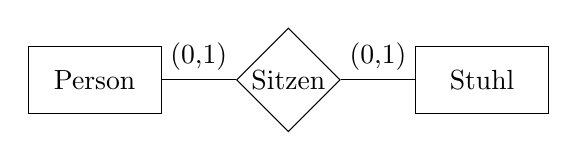
\begin{tikzpicture}[node  distance=7em]
      \node[entity] (person) {Person};
      \node[relationship] (sitzen) [right of=person] {Sitzen} edge node[above]{(0,1)} (person);
      \node[entity] (stuhl) [right of=sitzen] {Stuhl} edge node[above]{(0,1)} (sitzen);
    \end{tikzpicture}
  \end{figure}

  \todo[inline]{ggf.~zitieren: Datenmodelle, Datenbanksprachen und Datenbankmanagementsysteme
  von Gottfried Vossen}
  \todo[inline]{ERM als Thema zu allgemein? Nicht zum Seiten füllen!}
  \todo[inline]{Attribute auch erläutern}

  \section{Dimensions-Modell}
  Es gibt verschiedene Ausprägungen des Dimensions-Modells. Zunächst wird auf
  allgemeine Eigenschaften der Modell-Gruppe eingegangen.

  Im Mittelpunkt der Dimensions-Modellierung stehen die
  betriebswirtschaftlichen Fakten~\cite[][S.  2]{phipps2002automating}. Ein
  Fakt kann eine Transaktion, ein Objekt oder ein Ereignis sein~\cite[][S.
  42]{ballard1998data}. \textsc{\citeauthor{Kemper2010}} nennt als Beispiele:
  \glqq{}Umsatzerlöse, Umsatzmengen, Einzelkosten oder den
  Personalbedarf\grqq{}\cite[][S. 66]{Kemper2010}. 
  
  Um verschiedene Sichten auf diese Fakten zu erlangen, gruppiert man diese in
  Dimensionen \bzw{} weist ihnen Dimensionsausprägungen zu~\cite[][S.
  66]{Kemper2010}. Dies ermöglicht es, in der späteren Analyse nach
  verschiedenen Dimensionen zu filtern und zu vergleichen. Dimensionen werden
  hierarchisch strukturiert. Mit Hilfe der daraus entstehenden Hierarchiestufen
  kann die Sicht auf die Daten in ihrem Detailgrad angepasst werden~\cite[][S.
  66]{Kemper2010}. Wege innerhalb der Hierarchiestufen verlaufen nicht nur als
  einzelner Pfad linear, sondern auch als Graph. Ein Beispiel ist die
  Dimension \textit{Zeit}.  Diese kann zum einen durch die
  Hierarchiestufenreihe \textit{Jahr, Monat, Tag} als auch durch \textit{Jahr,
  Woche, Tag} strukturiert werden.

  Die Dimensions-Modellierung unterteilt sich nun in verschiedene Ausprägungen.
  Die bekannteste Ausprägung ist das Star-Modell~\cite[][S.
  2]{phipps2002automating}. Der Name ist zurück zu f\"uhren auf den Aufbau
  eines entsprechenden Modells (Siehe Abbildung~\ref{fig:star-schema}), welches
  die Form eines Sterns hat~\cite[][S.  44]{Kimball2013}. In der Mitte des
  Sterns befindet sich die Faktentabelle~\cite[][S. 67]{Kemper2010}. Diese
  verweist mit Hilfe von Fremdschlüsseln auf Dimensionstabellen, welche jeweils
  eine komplette Dimension abbilden und somit im Gegenzug auf die dritte
  Normalform verzichten~\cite[][S. 67 f.]{Kemper2010}. Die
  Datenredundanz (Siehe Abbildung~\ref{table:dimension-table}) in den
  Dimensionstabellen resultiert laut \textsc{\citeauthor{Kimball2013}} durch
  ihre geringe Größe nicht in einer schlechteren Leistung des Datenbanksystems,
  sondern im Gegenzug in einer besseren Verständlichkeit der
  Struktur~\cite[][S. 15]{Kimball2013}.

  \begin{figure}[caption={Star-Schema Beispielmodell angelehnt an~\cite{Kemper2010} Abb. 2.30}, label={fig:star-schema}]
    \resizebox{\columnwidth-90pt}{!}{% Graphic for TeX using PGF
% Title: /home/indenml/coding/bachelor_thesis/content/figures/star-schema.dia
% Creator: Dia v0.97.3
% CreationDate: Thu Aug  4 09:14:34 2016
% For: indenml
% \usepackage{tikz}
% The following commands are not supported in PSTricks at present
% We define them conditionally, so when they are implemented,
% this pgf file will use them.
\ifx\du\undefined
  \newlength{\du}
\fi
\setlength{\du}{15\unitlength}
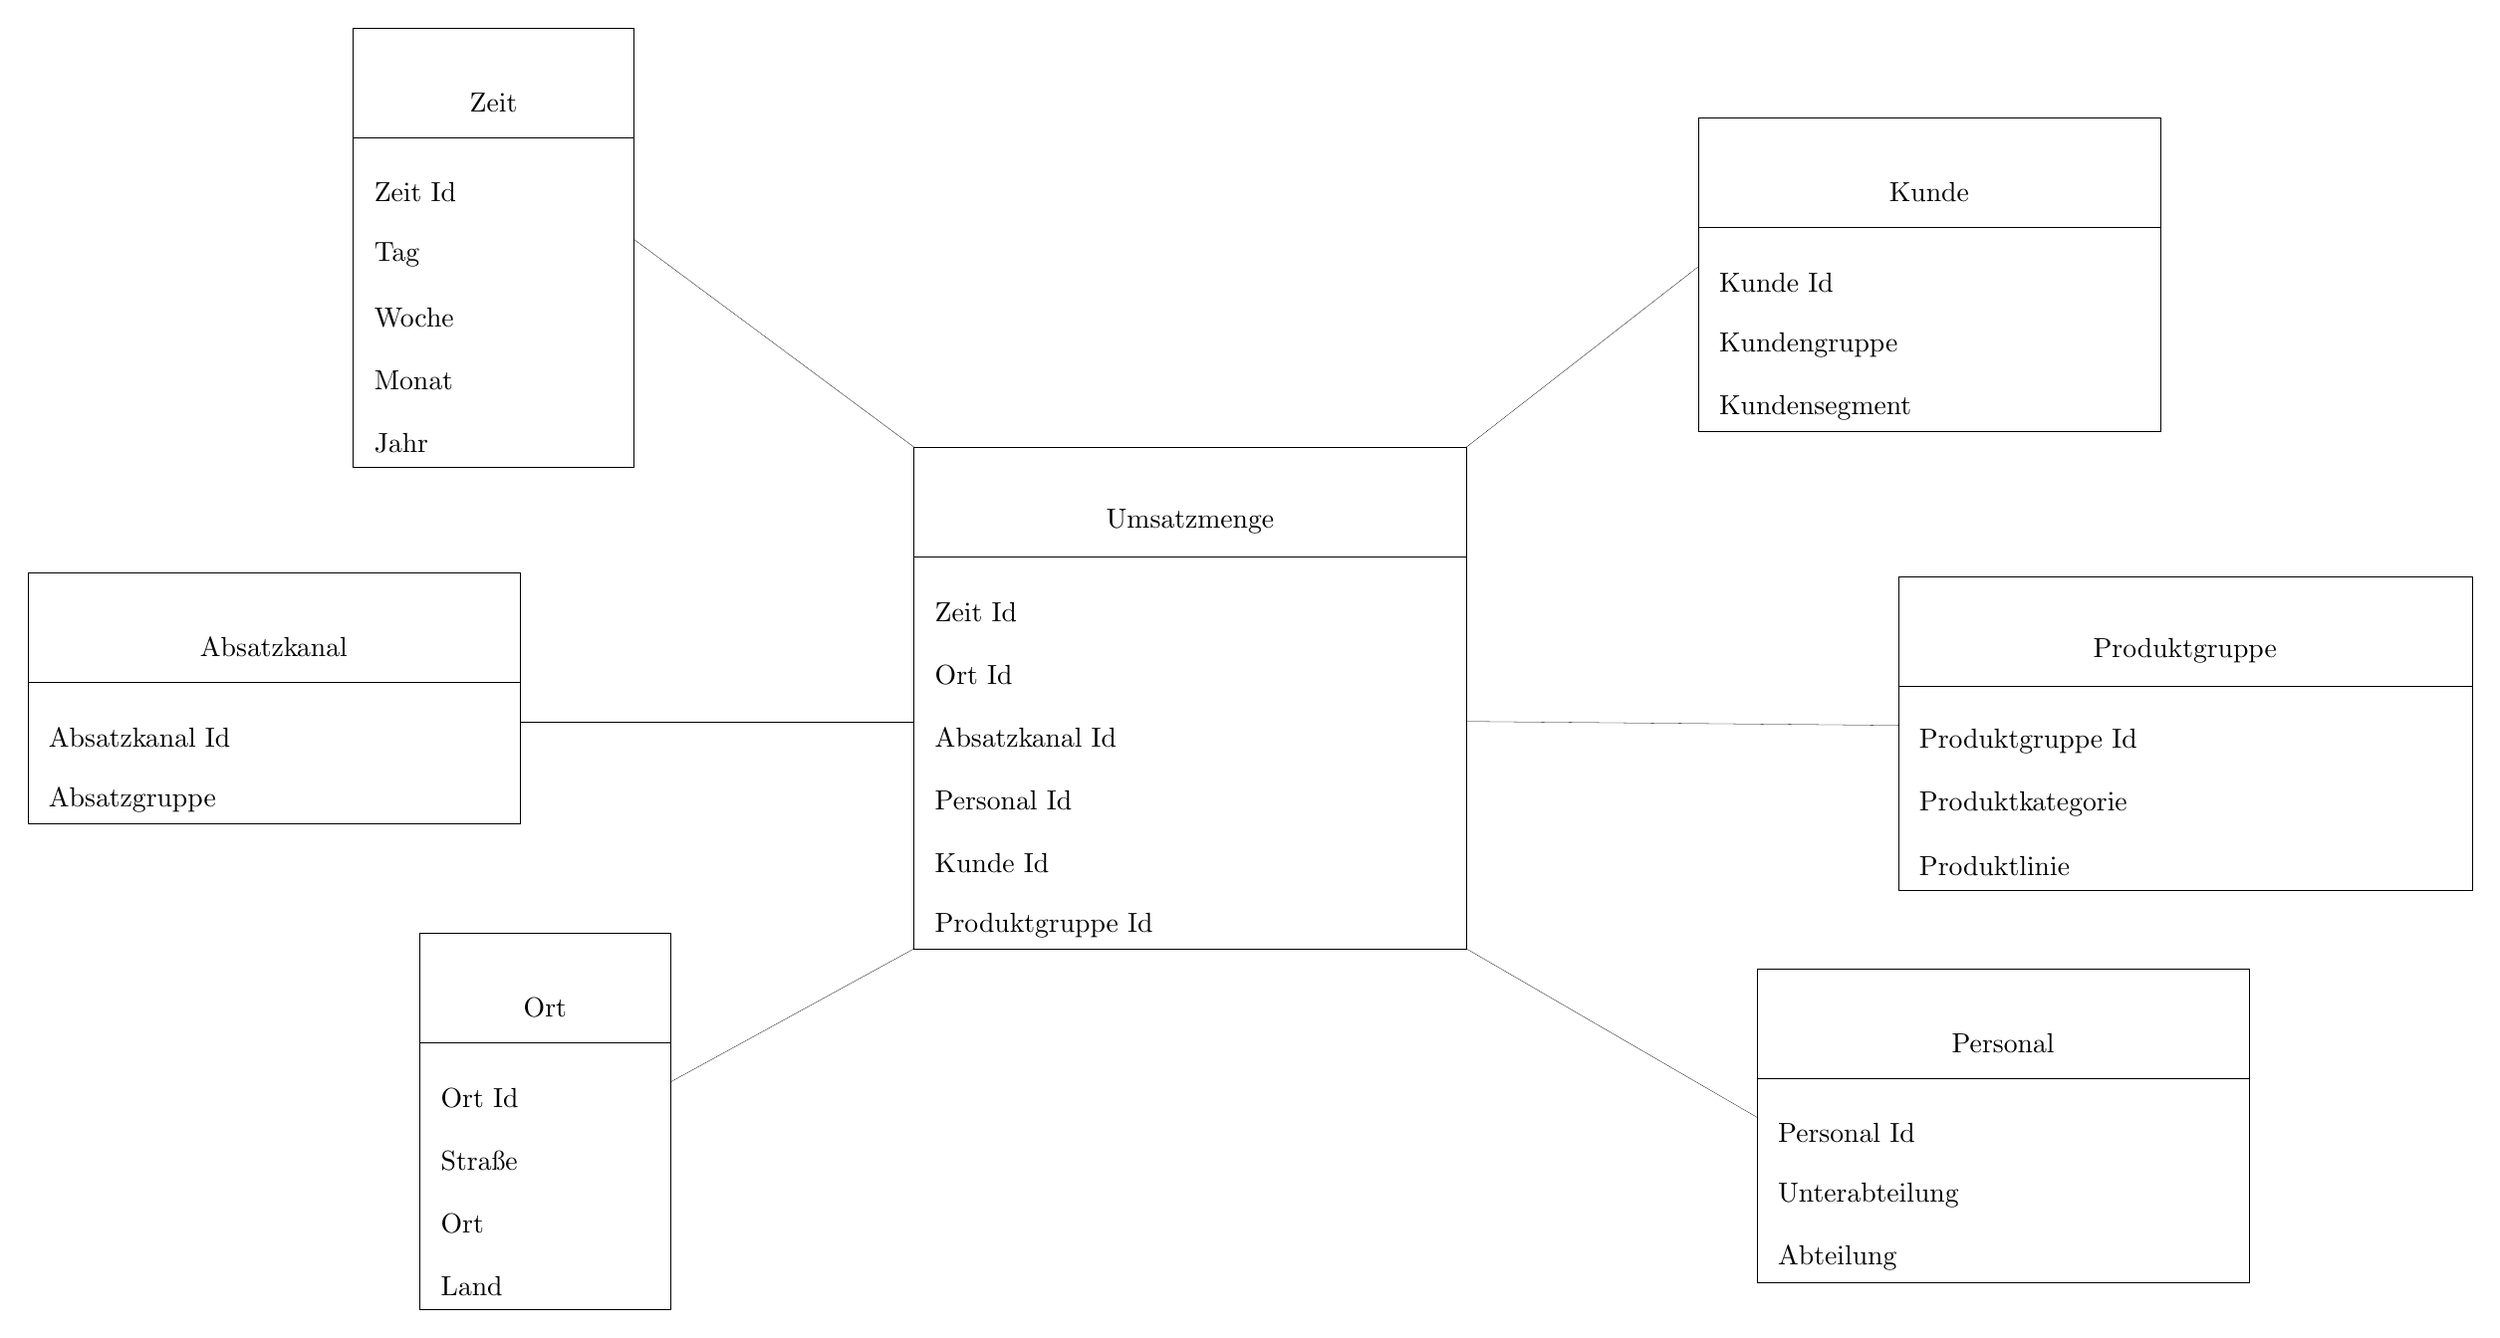
\begin{tikzpicture}
\pgftransformxscale{1.000000}
\pgftransformyscale{-1.000000}
\definecolor{dialinecolor}{rgb}{0.000000, 0.000000, 0.000000}
\pgfsetstrokecolor{dialinecolor}
\definecolor{dialinecolor}{rgb}{1.000000, 1.000000, 1.000000}
\pgfsetfillcolor{dialinecolor}
\pgfsetlinewidth{0.100000\du}
\pgfsetdash{}{0pt}
\definecolor{dialinecolor}{rgb}{1.000000, 1.000000, 1.000000}
\pgfsetfillcolor{dialinecolor}
\fill (23.000000\du,13.700000\du)--(23.000000\du,15.100000\du)--(30.045000\du,15.100000\du)--(30.045000\du,13.700000\du)--cycle;
\definecolor{dialinecolor}{rgb}{0.000000, 0.000000, 0.000000}
\pgfsetstrokecolor{dialinecolor}
\draw (23.000000\du,13.700000\du)--(23.000000\du,15.100000\du)--(30.045000\du,15.100000\du)--(30.045000\du,13.700000\du)--cycle;
% setfont left to latex
\definecolor{dialinecolor}{rgb}{0.000000, 0.000000, 0.000000}
\pgfsetstrokecolor{dialinecolor}
\node at (26.522500\du,14.650000\du){Umsatzmenge};
\definecolor{dialinecolor}{rgb}{1.000000, 1.000000, 1.000000}
\pgfsetfillcolor{dialinecolor}
\fill (23.000000\du,15.100000\du)--(23.000000\du,20.100000\du)--(30.045000\du,20.100000\du)--(30.045000\du,15.100000\du)--cycle;
\definecolor{dialinecolor}{rgb}{0.000000, 0.000000, 0.000000}
\pgfsetstrokecolor{dialinecolor}
\draw (23.000000\du,15.100000\du)--(23.000000\du,20.100000\du)--(30.045000\du,20.100000\du)--(30.045000\du,15.100000\du)--cycle;
% setfont left to latex
\definecolor{dialinecolor}{rgb}{0.000000, 0.000000, 0.000000}
\pgfsetstrokecolor{dialinecolor}
\node[anchor=west] at (23.150000\du,15.800000\du){ Zeit Id};
% setfont left to latex
\definecolor{dialinecolor}{rgb}{0.000000, 0.000000, 0.000000}
\pgfsetstrokecolor{dialinecolor}
\node[anchor=west] at (23.150000\du,16.600000\du){ Ort Id};
% setfont left to latex
\definecolor{dialinecolor}{rgb}{0.000000, 0.000000, 0.000000}
\pgfsetstrokecolor{dialinecolor}
\node[anchor=west] at (23.150000\du,17.400000\du){ Absatzkanal Id};
% setfont left to latex
\definecolor{dialinecolor}{rgb}{0.000000, 0.000000, 0.000000}
\pgfsetstrokecolor{dialinecolor}
\node[anchor=west] at (23.150000\du,18.200000\du){ Personal Id};
% setfont left to latex
\definecolor{dialinecolor}{rgb}{0.000000, 0.000000, 0.000000}
\pgfsetstrokecolor{dialinecolor}
\node[anchor=west] at (23.150000\du,19.000000\du){ Kunde Id};
% setfont left to latex
\definecolor{dialinecolor}{rgb}{0.000000, 0.000000, 0.000000}
\pgfsetstrokecolor{dialinecolor}
\node[anchor=west] at (23.150000\du,19.800000\du){ Produktgruppe Id};
\pgfsetlinewidth{0.100000\du}
\pgfsetdash{}{0pt}
\definecolor{dialinecolor}{rgb}{1.000000, 1.000000, 1.000000}
\pgfsetfillcolor{dialinecolor}
\fill (15.850000\du,8.350000\du)--(15.850000\du,9.750000\du)--(19.430000\du,9.750000\du)--(19.430000\du,8.350000\du)--cycle;
\definecolor{dialinecolor}{rgb}{0.000000, 0.000000, 0.000000}
\pgfsetstrokecolor{dialinecolor}
\draw (15.850000\du,8.350000\du)--(15.850000\du,9.750000\du)--(19.430000\du,9.750000\du)--(19.430000\du,8.350000\du)--cycle;
% setfont left to latex
\definecolor{dialinecolor}{rgb}{0.000000, 0.000000, 0.000000}
\pgfsetstrokecolor{dialinecolor}
\node at (17.640000\du,9.300000\du){Zeit};
\definecolor{dialinecolor}{rgb}{1.000000, 1.000000, 1.000000}
\pgfsetfillcolor{dialinecolor}
\fill (15.850000\du,9.750000\du)--(15.850000\du,13.950000\du)--(19.430000\du,13.950000\du)--(19.430000\du,9.750000\du)--cycle;
\definecolor{dialinecolor}{rgb}{0.000000, 0.000000, 0.000000}
\pgfsetstrokecolor{dialinecolor}
\draw (15.850000\du,9.750000\du)--(15.850000\du,13.950000\du)--(19.430000\du,13.950000\du)--(19.430000\du,9.750000\du)--cycle;
% setfont left to latex
\definecolor{dialinecolor}{rgb}{0.000000, 0.000000, 0.000000}
\pgfsetstrokecolor{dialinecolor}
\node[anchor=west] at (16.000000\du,10.450000\du){ Zeit Id};
% setfont left to latex
\definecolor{dialinecolor}{rgb}{0.000000, 0.000000, 0.000000}
\pgfsetstrokecolor{dialinecolor}
\node[anchor=west] at (16.000000\du,11.250000\du){ Tag};
% setfont left to latex
\definecolor{dialinecolor}{rgb}{0.000000, 0.000000, 0.000000}
\pgfsetstrokecolor{dialinecolor}
\node[anchor=west] at (16.000000\du,12.050000\du){ Woche};
% setfont left to latex
\definecolor{dialinecolor}{rgb}{0.000000, 0.000000, 0.000000}
\pgfsetstrokecolor{dialinecolor}
\node[anchor=west] at (16.000000\du,12.850000\du){ Monat};
% setfont left to latex
\definecolor{dialinecolor}{rgb}{0.000000, 0.000000, 0.000000}
\pgfsetstrokecolor{dialinecolor}
\node[anchor=west] at (16.000000\du,13.650000\du){ Jahr};
\pgfsetlinewidth{0.100000\du}
\pgfsetdash{}{0pt}
\definecolor{dialinecolor}{rgb}{1.000000, 1.000000, 1.000000}
\pgfsetfillcolor{dialinecolor}
\fill (16.700000\du,19.900000\du)--(16.700000\du,21.300000\du)--(19.895000\du,21.300000\du)--(19.895000\du,19.900000\du)--cycle;
\definecolor{dialinecolor}{rgb}{0.000000, 0.000000, 0.000000}
\pgfsetstrokecolor{dialinecolor}
\draw (16.700000\du,19.900000\du)--(16.700000\du,21.300000\du)--(19.895000\du,21.300000\du)--(19.895000\du,19.900000\du)--cycle;
% setfont left to latex
\definecolor{dialinecolor}{rgb}{0.000000, 0.000000, 0.000000}
\pgfsetstrokecolor{dialinecolor}
\node at (18.297500\du,20.850000\du){Ort};
\definecolor{dialinecolor}{rgb}{1.000000, 1.000000, 1.000000}
\pgfsetfillcolor{dialinecolor}
\fill (16.700000\du,21.300000\du)--(16.700000\du,24.700000\du)--(19.895000\du,24.700000\du)--(19.895000\du,21.300000\du)--cycle;
\definecolor{dialinecolor}{rgb}{0.000000, 0.000000, 0.000000}
\pgfsetstrokecolor{dialinecolor}
\draw (16.700000\du,21.300000\du)--(16.700000\du,24.700000\du)--(19.895000\du,24.700000\du)--(19.895000\du,21.300000\du)--cycle;
% setfont left to latex
\definecolor{dialinecolor}{rgb}{0.000000, 0.000000, 0.000000}
\pgfsetstrokecolor{dialinecolor}
\node[anchor=west] at (16.850000\du,22.000000\du){ Ort Id};
% setfont left to latex
\definecolor{dialinecolor}{rgb}{0.000000, 0.000000, 0.000000}
\pgfsetstrokecolor{dialinecolor}
\node[anchor=west] at (16.850000\du,22.800000\du){ Straße};
% setfont left to latex
\definecolor{dialinecolor}{rgb}{0.000000, 0.000000, 0.000000}
\pgfsetstrokecolor{dialinecolor}
\node[anchor=west] at (16.850000\du,23.600000\du){ Ort};
% setfont left to latex
\definecolor{dialinecolor}{rgb}{0.000000, 0.000000, 0.000000}
\pgfsetstrokecolor{dialinecolor}
\node[anchor=west] at (16.850000\du,24.400000\du){ Land};
\pgfsetlinewidth{0.100000\du}
\pgfsetdash{}{0pt}
\definecolor{dialinecolor}{rgb}{1.000000, 1.000000, 1.000000}
\pgfsetfillcolor{dialinecolor}
\fill (33.000000\du,9.500000\du)--(33.000000\du,10.900000\du)--(38.890000\du,10.900000\du)--(38.890000\du,9.500000\du)--cycle;
\definecolor{dialinecolor}{rgb}{0.000000, 0.000000, 0.000000}
\pgfsetstrokecolor{dialinecolor}
\draw (33.000000\du,9.500000\du)--(33.000000\du,10.900000\du)--(38.890000\du,10.900000\du)--(38.890000\du,9.500000\du)--cycle;
% setfont left to latex
\definecolor{dialinecolor}{rgb}{0.000000, 0.000000, 0.000000}
\pgfsetstrokecolor{dialinecolor}
\node at (35.945000\du,10.450000\du){Kunde};
\definecolor{dialinecolor}{rgb}{1.000000, 1.000000, 1.000000}
\pgfsetfillcolor{dialinecolor}
\fill (33.000000\du,10.900000\du)--(33.000000\du,13.500000\du)--(38.890000\du,13.500000\du)--(38.890000\du,10.900000\du)--cycle;
\definecolor{dialinecolor}{rgb}{0.000000, 0.000000, 0.000000}
\pgfsetstrokecolor{dialinecolor}
\draw (33.000000\du,10.900000\du)--(33.000000\du,13.500000\du)--(38.890000\du,13.500000\du)--(38.890000\du,10.900000\du)--cycle;
% setfont left to latex
\definecolor{dialinecolor}{rgb}{0.000000, 0.000000, 0.000000}
\pgfsetstrokecolor{dialinecolor}
\node[anchor=west] at (33.150000\du,11.600000\du){ Kunde Id};
% setfont left to latex
\definecolor{dialinecolor}{rgb}{0.000000, 0.000000, 0.000000}
\pgfsetstrokecolor{dialinecolor}
\node[anchor=west] at (33.150000\du,12.400000\du){ Kundengruppe};
% setfont left to latex
\definecolor{dialinecolor}{rgb}{0.000000, 0.000000, 0.000000}
\pgfsetstrokecolor{dialinecolor}
\node[anchor=west] at (33.150000\du,13.200000\du){ Kundensegment};
\pgfsetlinewidth{0.100000\du}
\pgfsetdash{}{0pt}
\definecolor{dialinecolor}{rgb}{1.000000, 1.000000, 1.000000}
\pgfsetfillcolor{dialinecolor}
\fill (33.750000\du,20.350000\du)--(33.750000\du,21.750000\du)--(40.025000\du,21.750000\du)--(40.025000\du,20.350000\du)--cycle;
\definecolor{dialinecolor}{rgb}{0.000000, 0.000000, 0.000000}
\pgfsetstrokecolor{dialinecolor}
\draw (33.750000\du,20.350000\du)--(33.750000\du,21.750000\du)--(40.025000\du,21.750000\du)--(40.025000\du,20.350000\du)--cycle;
% setfont left to latex
\definecolor{dialinecolor}{rgb}{0.000000, 0.000000, 0.000000}
\pgfsetstrokecolor{dialinecolor}
\node at (36.887500\du,21.300000\du){Personal};
\definecolor{dialinecolor}{rgb}{1.000000, 1.000000, 1.000000}
\pgfsetfillcolor{dialinecolor}
\fill (33.750000\du,21.750000\du)--(33.750000\du,24.350000\du)--(40.025000\du,24.350000\du)--(40.025000\du,21.750000\du)--cycle;
\definecolor{dialinecolor}{rgb}{0.000000, 0.000000, 0.000000}
\pgfsetstrokecolor{dialinecolor}
\draw (33.750000\du,21.750000\du)--(33.750000\du,24.350000\du)--(40.025000\du,24.350000\du)--(40.025000\du,21.750000\du)--cycle;
% setfont left to latex
\definecolor{dialinecolor}{rgb}{0.000000, 0.000000, 0.000000}
\pgfsetstrokecolor{dialinecolor}
\node[anchor=west] at (33.900000\du,22.450000\du){ Personal Id};
% setfont left to latex
\definecolor{dialinecolor}{rgb}{0.000000, 0.000000, 0.000000}
\pgfsetstrokecolor{dialinecolor}
\node[anchor=west] at (33.900000\du,23.250000\du){ Unterabteilung};
% setfont left to latex
\definecolor{dialinecolor}{rgb}{0.000000, 0.000000, 0.000000}
\pgfsetstrokecolor{dialinecolor}
\node[anchor=west] at (33.900000\du,24.050000\du){ Abteilung};
\pgfsetlinewidth{0.100000\du}
\pgfsetdash{}{0pt}
\definecolor{dialinecolor}{rgb}{1.000000, 1.000000, 1.000000}
\pgfsetfillcolor{dialinecolor}
\fill (11.700000\du,15.300000\du)--(11.700000\du,16.700000\du)--(17.975000\du,16.700000\du)--(17.975000\du,15.300000\du)--cycle;
\definecolor{dialinecolor}{rgb}{0.000000, 0.000000, 0.000000}
\pgfsetstrokecolor{dialinecolor}
\draw (11.700000\du,15.300000\du)--(11.700000\du,16.700000\du)--(17.975000\du,16.700000\du)--(17.975000\du,15.300000\du)--cycle;
% setfont left to latex
\definecolor{dialinecolor}{rgb}{0.000000, 0.000000, 0.000000}
\pgfsetstrokecolor{dialinecolor}
\node at (14.837500\du,16.250000\du){Absatzkanal};
\definecolor{dialinecolor}{rgb}{1.000000, 1.000000, 1.000000}
\pgfsetfillcolor{dialinecolor}
\fill (11.700000\du,16.700000\du)--(11.700000\du,18.500000\du)--(17.975000\du,18.500000\du)--(17.975000\du,16.700000\du)--cycle;
\definecolor{dialinecolor}{rgb}{0.000000, 0.000000, 0.000000}
\pgfsetstrokecolor{dialinecolor}
\draw (11.700000\du,16.700000\du)--(11.700000\du,18.500000\du)--(17.975000\du,18.500000\du)--(17.975000\du,16.700000\du)--cycle;
% setfont left to latex
\definecolor{dialinecolor}{rgb}{0.000000, 0.000000, 0.000000}
\pgfsetstrokecolor{dialinecolor}
\node[anchor=west] at (11.850000\du,17.400000\du){ Absatzkanal Id};
% setfont left to latex
\definecolor{dialinecolor}{rgb}{0.000000, 0.000000, 0.000000}
\pgfsetstrokecolor{dialinecolor}
\node[anchor=west] at (11.850000\du,18.200000\du){ Absatzgruppe};
\pgfsetlinewidth{0.100000\du}
\pgfsetdash{}{0pt}
\definecolor{dialinecolor}{rgb}{1.000000, 1.000000, 1.000000}
\pgfsetfillcolor{dialinecolor}
\fill (35.550000\du,15.350000\du)--(35.550000\du,16.750000\du)--(42.865000\du,16.750000\du)--(42.865000\du,15.350000\du)--cycle;
\definecolor{dialinecolor}{rgb}{0.000000, 0.000000, 0.000000}
\pgfsetstrokecolor{dialinecolor}
\draw (35.550000\du,15.350000\du)--(35.550000\du,16.750000\du)--(42.865000\du,16.750000\du)--(42.865000\du,15.350000\du)--cycle;
% setfont left to latex
\definecolor{dialinecolor}{rgb}{0.000000, 0.000000, 0.000000}
\pgfsetstrokecolor{dialinecolor}
\node at (39.207500\du,16.300000\du){Produktgruppe};
\definecolor{dialinecolor}{rgb}{1.000000, 1.000000, 1.000000}
\pgfsetfillcolor{dialinecolor}
\fill (35.550000\du,16.750000\du)--(35.550000\du,19.350000\du)--(42.865000\du,19.350000\du)--(42.865000\du,16.750000\du)--cycle;
\definecolor{dialinecolor}{rgb}{0.000000, 0.000000, 0.000000}
\pgfsetstrokecolor{dialinecolor}
\draw (35.550000\du,16.750000\du)--(35.550000\du,19.350000\du)--(42.865000\du,19.350000\du)--(42.865000\du,16.750000\du)--cycle;
% setfont left to latex
\definecolor{dialinecolor}{rgb}{0.000000, 0.000000, 0.000000}
\pgfsetstrokecolor{dialinecolor}
\node[anchor=west] at (35.700000\du,17.450000\du){ Produktgruppe Id};
% setfont left to latex
\definecolor{dialinecolor}{rgb}{0.000000, 0.000000, 0.000000}
\pgfsetstrokecolor{dialinecolor}
\node[anchor=west] at (35.700000\du,18.250000\du){ Produktkategorie};
% setfont left to latex
\definecolor{dialinecolor}{rgb}{0.000000, 0.000000, 0.000000}
\pgfsetstrokecolor{dialinecolor}
\node[anchor=west] at (35.700000\du,19.050000\du){ Produktlinie};
\pgfsetlinewidth{0.100000\du}
\pgfsetdash{}{0pt}
\pgfsetdash{}{0pt}
\pgfsetbuttcap
{
\definecolor{dialinecolor}{rgb}{0.000000, 0.000000, 0.000000}
\pgfsetfillcolor{dialinecolor}
% was here!!!
\definecolor{dialinecolor}{rgb}{0.000000, 0.000000, 0.000000}
\pgfsetstrokecolor{dialinecolor}
\draw (30.045000\du,17.200000\du)--(35.550000\du,17.250000\du);
}
\pgfsetlinewidth{0.100000\du}
\pgfsetdash{}{0pt}
\pgfsetdash{}{0pt}
\pgfsetbuttcap
{
\definecolor{dialinecolor}{rgb}{0.000000, 0.000000, 0.000000}
\pgfsetfillcolor{dialinecolor}
% was here!!!
\definecolor{dialinecolor}{rgb}{0.000000, 0.000000, 0.000000}
\pgfsetstrokecolor{dialinecolor}
\draw (19.895000\du,21.800000\du)--(23.000000\du,20.100000\du);
}
\pgfsetlinewidth{0.100000\du}
\pgfsetdash{}{0pt}
\pgfsetdash{}{0pt}
\pgfsetbuttcap
{
\definecolor{dialinecolor}{rgb}{0.000000, 0.000000, 0.000000}
\pgfsetfillcolor{dialinecolor}
% was here!!!
\definecolor{dialinecolor}{rgb}{0.000000, 0.000000, 0.000000}
\pgfsetstrokecolor{dialinecolor}
\draw (17.975000\du,17.200000\du)--(23.000000\du,17.200000\du);
}
\pgfsetlinewidth{0.100000\du}
\pgfsetdash{}{0pt}
\pgfsetdash{}{0pt}
\pgfsetbuttcap
{
\definecolor{dialinecolor}{rgb}{0.000000, 0.000000, 0.000000}
\pgfsetfillcolor{dialinecolor}
% was here!!!
\definecolor{dialinecolor}{rgb}{0.000000, 0.000000, 0.000000}
\pgfsetstrokecolor{dialinecolor}
\draw (30.045000\du,13.700000\du)--(33.000000\du,11.400000\du);
}
\pgfsetlinewidth{0.100000\du}
\pgfsetdash{}{0pt}
\pgfsetdash{}{0pt}
\pgfsetbuttcap
{
\definecolor{dialinecolor}{rgb}{0.000000, 0.000000, 0.000000}
\pgfsetfillcolor{dialinecolor}
% was here!!!
\definecolor{dialinecolor}{rgb}{0.000000, 0.000000, 0.000000}
\pgfsetstrokecolor{dialinecolor}
\draw (33.750000\du,22.250000\du)--(30.045000\du,20.100000\du);
}
\pgfsetlinewidth{0.100000\du}
\pgfsetdash{}{0pt}
\pgfsetdash{}{0pt}
\pgfsetbuttcap
{
\definecolor{dialinecolor}{rgb}{0.000000, 0.000000, 0.000000}
\pgfsetfillcolor{dialinecolor}
% was here!!!
\definecolor{dialinecolor}{rgb}{0.000000, 0.000000, 0.000000}
\pgfsetstrokecolor{dialinecolor}
\draw (19.430000\du,11.050000\du)--(23.000000\du,13.700000\du);
}
\end{tikzpicture}
}
  \end{figure}

  \todo{Soll ich erklären, dass die Tabelle nicht normalisiert ist?}
  \begin{figure}[caption={Beispiel der Dimensionstabelle \textit{Ort} im Star-Schema}, label={table:dimension-table}]
    \begin{tabular}{c c c c}
      Ort Id & Straße & Ort & Land \\
      \toprule
      0 & Corrensstraße & Münster & Deutschland \\
      1 & Rudolf-Harbig-Weg & Münster & Deutschland \\
      2 & Hauptstraße & Bonn & Deutschland \\
    \end{tabular}
  \end{figure}

  Eine weitere Ausprägung der Dimensions-Modellierung ist das Snowflake-Modell.
  Analog zum Star-Modell gleicht die Form eines Snowflake-Modells einer
  Schneeflocke~\cite[][S. 70]{Kemper2010}. Star- und Snowflake-Modell
  unterscheiden sich in der Datenhaltung der Dimensionstabellen. Wie bereits im
  vorherigen Absatz beschrieben verfolgt das Star-Schema einen denormalisierten
  Ansatz, wohin gegen die Dimensionstabellen des Snowflak-Modells normalisiert
  sind~\cite[][S. 70]{Kemper2010}. \textsc{\citeauthor{Kemper2010}} schlägt
  jedoch nicht den Ansatz der vollen Normalisierung vor, sondern eine
  geschwindigkeitsorientierte Teilnormalisierung~\cite[][S. 70]{Kemper2010}.
  \textsc{\citeauthor{Kimball2013}} hingegen rät komplett vom Snowflake-Modell
  ab, da es seiner Meinung nach sowohl die Verständlichkeit als auch \ggf{} die
  Geschwindigkeit negativ beeinträchtigt~\cite[][S. 50]{Kimball2013}.
  \todo[inline]{Grafiken als Beispiel wie beim Star-Modell}

  \begin{figure}[caption={Teilausschnitt eines Snowflake-Schema}, label={fig:snowflake-schema}]
    \resizebox{400pt}{!}{% Graphic for TeX using PGF
% Title: /home/indenml/coding/bachelor_thesis/content/figures/snowflake-schema.dia
% Creator: Dia v0.97.3
% CreationDate: Thu Aug 11 17:57:36 2016
% For: indenml
% \usepackage{tikz}
% The following commands are not supported in PSTricks at present
% We define them conditionally, so when they are implemented,
% this pgf file will use them.
\ifx\du\undefined
  \newlength{\du}
\fi
\setlength{\du}{15\unitlength}
\begin{tikzpicture}
\pgftransformxscale{1.000000}
\pgftransformyscale{-1.000000}
\definecolor{dialinecolor}{rgb}{0.000000, 0.000000, 0.000000}
\pgfsetstrokecolor{dialinecolor}
\definecolor{dialinecolor}{rgb}{1.000000, 1.000000, 1.000000}
\pgfsetfillcolor{dialinecolor}
\pgfsetlinewidth{0.100000\du}
\pgfsetdash{}{0pt}
\definecolor{dialinecolor}{rgb}{1.000000, 1.000000, 1.000000}
\pgfsetfillcolor{dialinecolor}
\fill (23.150000\du,13.700000\du)--(23.150000\du,15.100000\du)--(30.055000\du,15.100000\du)--(30.055000\du,13.700000\du)--cycle;
\definecolor{dialinecolor}{rgb}{0.000000, 0.000000, 0.000000}
\pgfsetstrokecolor{dialinecolor}
\draw (23.150000\du,13.700000\du)--(23.150000\du,15.100000\du)--(30.055000\du,15.100000\du)--(30.055000\du,13.700000\du)--cycle;
% setfont left to latex
\definecolor{dialinecolor}{rgb}{0.000000, 0.000000, 0.000000}
\pgfsetstrokecolor{dialinecolor}
\node at (26.602500\du,14.650000\du){Umsatzmenge};
\definecolor{dialinecolor}{rgb}{1.000000, 1.000000, 1.000000}
\pgfsetfillcolor{dialinecolor}
\fill (23.150000\du,15.100000\du)--(23.150000\du,20.900000\du)--(30.055000\du,20.900000\du)--(30.055000\du,15.100000\du)--cycle;
\definecolor{dialinecolor}{rgb}{0.000000, 0.000000, 0.000000}
\pgfsetstrokecolor{dialinecolor}
\draw (23.150000\du,15.100000\du)--(23.150000\du,20.900000\du)--(30.055000\du,20.900000\du)--(30.055000\du,15.100000\du)--cycle;
% setfont left to latex
\definecolor{dialinecolor}{rgb}{0.000000, 0.000000, 0.000000}
\pgfsetstrokecolor{dialinecolor}
\node[anchor=west] at (23.300000\du,15.800000\du){ Zeit Id};
% setfont left to latex
\definecolor{dialinecolor}{rgb}{0.000000, 0.000000, 0.000000}
\pgfsetstrokecolor{dialinecolor}
\node[anchor=west] at (23.300000\du,16.600000\du){ Straße Id};
% setfont left to latex
\definecolor{dialinecolor}{rgb}{0.000000, 0.000000, 0.000000}
\pgfsetstrokecolor{dialinecolor}
\node[anchor=west] at (23.300000\du,17.400000\du){ Absatzkanal Id};
% setfont left to latex
\definecolor{dialinecolor}{rgb}{0.000000, 0.000000, 0.000000}
\pgfsetstrokecolor{dialinecolor}
\node[anchor=west] at (23.300000\du,18.200000\du){ Personal Id};
% setfont left to latex
\definecolor{dialinecolor}{rgb}{0.000000, 0.000000, 0.000000}
\pgfsetstrokecolor{dialinecolor}
\node[anchor=west] at (23.300000\du,19.000000\du){ Kunde Id};
% setfont left to latex
\definecolor{dialinecolor}{rgb}{0.000000, 0.000000, 0.000000}
\pgfsetstrokecolor{dialinecolor}
\node[anchor=west] at (23.300000\du,19.800000\du){ Produkt Id};
% setfont left to latex
\definecolor{dialinecolor}{rgb}{0.000000, 0.000000, 0.000000}
\pgfsetstrokecolor{dialinecolor}
\node[anchor=west] at (23.300000\du,20.600000\du){ };
\pgfsetlinewidth{0.100000\du}
\pgfsetdash{}{0pt}
\definecolor{dialinecolor}{rgb}{1.000000, 1.000000, 1.000000}
\pgfsetfillcolor{dialinecolor}
\fill (16.700000\du,15.297000\du)--(16.700000\du,16.697000\du)--(21.050000\du,16.697000\du)--(21.050000\du,15.297000\du)--cycle;
\definecolor{dialinecolor}{rgb}{0.000000, 0.000000, 0.000000}
\pgfsetstrokecolor{dialinecolor}
\draw (16.700000\du,15.297000\du)--(16.700000\du,16.697000\du)--(21.050000\du,16.697000\du)--(21.050000\du,15.297000\du)--cycle;
% setfont left to latex
\definecolor{dialinecolor}{rgb}{0.000000, 0.000000, 0.000000}
\pgfsetstrokecolor{dialinecolor}
\node at (18.875000\du,16.247000\du){Straße};
\definecolor{dialinecolor}{rgb}{1.000000, 1.000000, 1.000000}
\pgfsetfillcolor{dialinecolor}
\fill (16.700000\du,16.697000\du)--(16.700000\du,20.097000\du)--(21.050000\du,20.097000\du)--(21.050000\du,16.697000\du)--cycle;
\definecolor{dialinecolor}{rgb}{0.000000, 0.000000, 0.000000}
\pgfsetstrokecolor{dialinecolor}
\draw (16.700000\du,16.697000\du)--(16.700000\du,20.097000\du)--(21.050000\du,20.097000\du)--(21.050000\du,16.697000\du)--cycle;
% setfont left to latex
\definecolor{dialinecolor}{rgb}{0.000000, 0.000000, 0.000000}
\pgfsetstrokecolor{dialinecolor}
\node[anchor=west] at (16.850000\du,17.397000\du){ Straße Id};
% setfont left to latex
\definecolor{dialinecolor}{rgb}{0.000000, 0.000000, 0.000000}
\pgfsetstrokecolor{dialinecolor}
\node[anchor=west] at (16.850000\du,18.197000\du){ Name};
% setfont left to latex
\definecolor{dialinecolor}{rgb}{0.000000, 0.000000, 0.000000}
\pgfsetstrokecolor{dialinecolor}
\node[anchor=west] at (16.850000\du,18.997000\du){ Ort Id};
% setfont left to latex
\definecolor{dialinecolor}{rgb}{0.000000, 0.000000, 0.000000}
\pgfsetstrokecolor{dialinecolor}
\node[anchor=west] at (16.850000\du,19.797000\du){ };
\pgfsetlinewidth{0.100000\du}
\pgfsetdash{}{0pt}
\pgfsetdash{}{0pt}
\pgfsetbuttcap
{
\definecolor{dialinecolor}{rgb}{0.000000, 0.000000, 0.000000}
\pgfsetfillcolor{dialinecolor}
% was here!!!
\definecolor{dialinecolor}{rgb}{0.000000, 0.000000, 0.000000}
\pgfsetstrokecolor{dialinecolor}
\draw (21.050000\du,17.197000\du)--(23.150000\du,17.200000\du);
}
\pgfsetlinewidth{0.100000\du}
\pgfsetdash{}{0pt}
\definecolor{dialinecolor}{rgb}{1.000000, 1.000000, 1.000000}
\pgfsetfillcolor{dialinecolor}
\fill (5.855000\du,15.307100\du)--(5.855000\du,16.707100\du)--(9.435000\du,16.707100\du)--(9.435000\du,15.307100\du)--cycle;
\definecolor{dialinecolor}{rgb}{0.000000, 0.000000, 0.000000}
\pgfsetstrokecolor{dialinecolor}
\draw (5.855000\du,15.307100\du)--(5.855000\du,16.707100\du)--(9.435000\du,16.707100\du)--(9.435000\du,15.307100\du)--cycle;
% setfont left to latex
\definecolor{dialinecolor}{rgb}{0.000000, 0.000000, 0.000000}
\pgfsetstrokecolor{dialinecolor}
\node at (7.645000\du,16.257100\du){Land};
\definecolor{dialinecolor}{rgb}{1.000000, 1.000000, 1.000000}
\pgfsetfillcolor{dialinecolor}
\fill (5.855000\du,16.707100\du)--(5.855000\du,19.307100\du)--(9.435000\du,19.307100\du)--(9.435000\du,16.707100\du)--cycle;
\definecolor{dialinecolor}{rgb}{0.000000, 0.000000, 0.000000}
\pgfsetstrokecolor{dialinecolor}
\draw (5.855000\du,16.707100\du)--(5.855000\du,19.307100\du)--(9.435000\du,19.307100\du)--(9.435000\du,16.707100\du)--cycle;
% setfont left to latex
\definecolor{dialinecolor}{rgb}{0.000000, 0.000000, 0.000000}
\pgfsetstrokecolor{dialinecolor}
\node[anchor=west] at (6.005000\du,17.407100\du){ Land Id};
% setfont left to latex
\definecolor{dialinecolor}{rgb}{0.000000, 0.000000, 0.000000}
\pgfsetstrokecolor{dialinecolor}
\node[anchor=west] at (6.005000\du,18.207100\du){ Name};
% setfont left to latex
\definecolor{dialinecolor}{rgb}{0.000000, 0.000000, 0.000000}
\pgfsetstrokecolor{dialinecolor}
\node[anchor=west] at (6.005000\du,19.007100\du){ };
\pgfsetlinewidth{0.100000\du}
\pgfsetdash{}{0pt}
\definecolor{dialinecolor}{rgb}{1.000000, 1.000000, 1.000000}
\pgfsetfillcolor{dialinecolor}
\fill (11.260000\du,15.297500\du)--(11.260000\du,16.697500\du)--(14.840000\du,16.697500\du)--(14.840000\du,15.297500\du)--cycle;
\definecolor{dialinecolor}{rgb}{0.000000, 0.000000, 0.000000}
\pgfsetstrokecolor{dialinecolor}
\draw (11.260000\du,15.297500\du)--(11.260000\du,16.697500\du)--(14.840000\du,16.697500\du)--(14.840000\du,15.297500\du)--cycle;
% setfont left to latex
\definecolor{dialinecolor}{rgb}{0.000000, 0.000000, 0.000000}
\pgfsetstrokecolor{dialinecolor}
\node at (13.050000\du,16.247500\du){Ort};
\definecolor{dialinecolor}{rgb}{1.000000, 1.000000, 1.000000}
\pgfsetfillcolor{dialinecolor}
\fill (11.260000\du,16.697500\du)--(11.260000\du,20.097500\du)--(14.840000\du,20.097500\du)--(14.840000\du,16.697500\du)--cycle;
\definecolor{dialinecolor}{rgb}{0.000000, 0.000000, 0.000000}
\pgfsetstrokecolor{dialinecolor}
\draw (11.260000\du,16.697500\du)--(11.260000\du,20.097500\du)--(14.840000\du,20.097500\du)--(14.840000\du,16.697500\du)--cycle;
% setfont left to latex
\definecolor{dialinecolor}{rgb}{0.000000, 0.000000, 0.000000}
\pgfsetstrokecolor{dialinecolor}
\node[anchor=west] at (11.410000\du,17.397500\du){ Ort Id};
% setfont left to latex
\definecolor{dialinecolor}{rgb}{0.000000, 0.000000, 0.000000}
\pgfsetstrokecolor{dialinecolor}
\node[anchor=west] at (11.410000\du,18.197500\du){ Name};
% setfont left to latex
\definecolor{dialinecolor}{rgb}{0.000000, 0.000000, 0.000000}
\pgfsetstrokecolor{dialinecolor}
\node[anchor=west] at (11.410000\du,18.997500\du){ Land Id};
% setfont left to latex
\definecolor{dialinecolor}{rgb}{0.000000, 0.000000, 0.000000}
\pgfsetstrokecolor{dialinecolor}
\node[anchor=west] at (11.410000\du,19.797500\du){ };
\pgfsetlinewidth{0.100000\du}
\pgfsetdash{}{0pt}
\pgfsetdash{}{0pt}
\pgfsetbuttcap
{
\definecolor{dialinecolor}{rgb}{0.000000, 0.000000, 0.000000}
\pgfsetfillcolor{dialinecolor}
% was here!!!
\definecolor{dialinecolor}{rgb}{0.000000, 0.000000, 0.000000}
\pgfsetstrokecolor{dialinecolor}
\draw (14.840000\du,17.197500\du)--(16.700000\du,17.197000\du);
}
\pgfsetlinewidth{0.100000\du}
\pgfsetdash{}{0pt}
\pgfsetdash{}{0pt}
\pgfsetbuttcap
{
\definecolor{dialinecolor}{rgb}{0.000000, 0.000000, 0.000000}
\pgfsetfillcolor{dialinecolor}
% was here!!!
\definecolor{dialinecolor}{rgb}{0.000000, 0.000000, 0.000000}
\pgfsetstrokecolor{dialinecolor}
\draw (9.435000\du,17.207100\du)--(11.260000\du,17.197500\du);
}
\end{tikzpicture}
}
  \end{figure}

  \begin{figure}[caption={Beispiel der Dimensionstabellen \textit{Ort} im Snowflake-Schema}, label={table:dimension-table}]
    \begin{tabular}{c c c }
      Straße Id & Name & Ort Id \\
      \toprule
      0 & Corrensstraße & 0 \\
      1 & Rudolf-Harbig-Weg & 0 \\
      2 & Hauptstraße & 1 \\
    \end{tabular}
    \begin{tabular}{c c c}
      Ort Id & Name & Land \\
      \toprule
      0 & Münster & 0 \\
      1 & Bonn & 0 \\
    \end{tabular}
    \begin{tabular}{c c c }
      Land Id & Name \\
      \toprule
      0 & Deutschland \\
      1 & Frankreich \\
    \end{tabular}
  \end{figure}

  \section{Vergleich ER-Modell und Dimensions-Modell}
  \textsc{\citeauthor{ballard1998data}} bezeichnet die Dimensions-Modellierung
  als Obermenge der ER-Modellierung~\cite[][S. 47]{ballard1998data}. Die
  Dimensions-Modellierung kann laut \textsc{\citeauthor{ballard1998data}}
  mittels der Notation der ER-Modellierung visualisiert werden~\cite[][S.
  47]{ballard1998data}. Zum Beispiel können die Fakten eines Dimensions-Modells
  als Objekte eines ER-Modells mit Beziehungen zu den jeweiligen Dimensionen,
  wiederum als Objekt, modelliert werden~\cite[][S. 48]{ballard1998data}. 

  \acrlong{OLTP}-Systeme (OLTP) sind operative Echtzeitsysteme mit dem
  spezifischen Fokus auf Transaktionsdaten des Tagesgeschäfts~\cite[][S.
  11]{gabriel2009data}. \acrlong{OLAP}-Systeme (OLAP) sind analytische Systeme,
  welche mit aufbereiteten, historischen Daten in Entscheidungsprozessen der
  Unternehmensführung helfen sollen~\cite[][S. 1]{chaudhuri1997overview}. Die
  Anwendungsbereiche der beiden Systeme sind disjunkt~\cite[][S.
  334]{chamoni2000line}. Nach \textsc{\citeauthor{phipps2002automating}} wird
  im Umgang mit \acrshort{OLTP}-Systemen überwiegend auf die ER-Modellierung
  zurück gegriffen, wo hingegen \acrshort{OLAP}-Systeme meist mit der
  Dimensions-Modellierung konzipiert werden~\cite[][S.
  2]{phipps2002automating}. 

  Systeme, welche nach der ER-Modellierung entwickelt wurden und einer strengen
  Normalisierung folgen, können zwar vergleichbar schnelle Einfüge-, Änder- und
  Löschoperationen durchführen, jedoch weisen sie bei großen Datensätzen und
  komplizierten Anfragen eine langsame Verarbeitung auf~\cite[][S.
  52]{ballard2012dimensional}. Mit der Dimensions-Modellierung können diese
  Anfragen schneller verarbeitet werden\cite[][S.  52]{ballard2012dimensional},
  unter anderem zurück zu führen auf die geringere Normalisierung, wodurch
  sich die Dimensions-Modellierung gegenüber der ER-Modellierung für \acrshort{OLAP}-Systeme besser eignet.


  \section{Erweiterung der Dimensions-Modellierung---H2 for Reporting}
  Die Dimensions-Modellierung wird durch verschiedene Modellierungssprachen
  erweitert. Hierzu zählt \zB{} \textit{H2 for Reporting}, entwickelt vom
  Institut für Wirtschaftsinformatik an der \acrlong{WWU} (WWU)
  Münster\todo{Stimmt das und wenn ja belegen!}. \textit{H2 for Reporting}
  ergänzt die Dimensions-Modellierung unter anderem um Bezugsobjekte,
  Kennzahlen und Berichte:
  \begin{itemize}
    \item Bezugsobjekte bilden die
      Basisobjekte der Datenanalyse, Beispiele sind Ort, Zeit oder
      Produkt~\cite[][S.  5]{becker2007h2}. 
    \item Kennzahlen ermöglichen die qualitative
      und quantitative Teilanalyse von Bezugsobjekten. Sie werden unterschieden in
      Basiskennzahlen und berechneten \todo{berechnende oder berechnete} Kennzahlen, welche wiederum in Kennzahlen mit
      Bezug auf ein und mit Bezug auf mehrere Objekte unterteilt werden~\cite[][S.
      15]{becker2007h2}. \textsc{\citeauthor{becker2007h2}} nennt als Beispiel
      einer berechnenden Kennzahl den Umsatz~\cite[][S. 17]{becker2007h2}.
    \item Berichte dienen der Visualisierung von Erkenntnissen aus der Kombination von
      Bezugsobjekten, Dimensionen und Kennzahlen und können zum Beispiel mit der
      Hilfe einer Tabelle abgebildet werden~\cite[][S. 23]{becker2007h2}.
  \end{itemize}

  Für die Anwendung von \textit{H2 for Reporting} kann das
  Metamodellierungswerkzeug \textit{H2-Toolset} verwendet werden~\cite[][S.
  33]{fleischer2013konstruktion}. Dieses wurde ebenfalls an der
  \acrshort{WWU}-Münster entwickelt~\cite[][S. 34]{becker2007h2}.

  \begin{itemize}
    \item H2 for Reporting
    \item Cognos
    \item Palos
    \item IBM
    \item Firmen Cognos, SAP, MicroStrategy oder BusinessObjects
  \end{itemize}

  \paragraph{Beispielszenario}
  Für den weiteren Verlauf dieser Arbeit wird ein Beispielszenario aufgestellt. Im
  Fokus steht eine fiktive Firma namens SmartSell. SmartSell setzt seine
  Produkte sowohl klassisch über ihr lokales Geschäft, als auch über einen
  eigenen Online-Shop ab.

  Beispiel Dimensionen
  \begin{itemize}
    \item Absatzkanal
    \item Zeit
    \item Produkt
    \item Ort
    \item Kunde
    \item Personal
    \item Lieferant
    \item Wertansatz (Soll, Ist, Plan)
  \end{itemize}


  % ################################################################################
  \chapter{DataFurnace-Sprache für innoscale}
  % ################################################################################

  \texthl{Ein Subset von H2ForReporting? F\"ur DQM statt f\"ur Business Intelligence?}

  \section{Anforderungsanalyse und Annahmen}
  Die Sprache ist bewusst schlicht gehalten um mit dem Ziel von DataRocket,
  \acrshort{DQM} IT-Laien zu ermöglichen, kohärent zu bleiben.

  \todo{Was mit der doppelten entity Ausprägung machen?}
  \section{Fachliches Konzept der Sprache}
  \begin{figure}[caption={Metamodell der DataFurnace-Sprache}, label={fig:img01}]
    \resizebox{\columnwidth}{!}{% Graphic for TeX using PGF
% Title: /home/indenml/ownCloud/wwu_wi/s6/bachelorarbeit/graphics/object-erm.dia
% Creator: Dia v0.97.3
% CreationDate: Thu Jul 21 15:40:48 2016
% For: indenml
% \usepackage{tikz}
% The following commands are not supported in PSTricks at present
% We define them conditionally, so when they are implemented,
% this pgf file will use them.
\ifx\du\undefined
  \newlength{\du}
\fi
\setlength{\du}{15\unitlength}
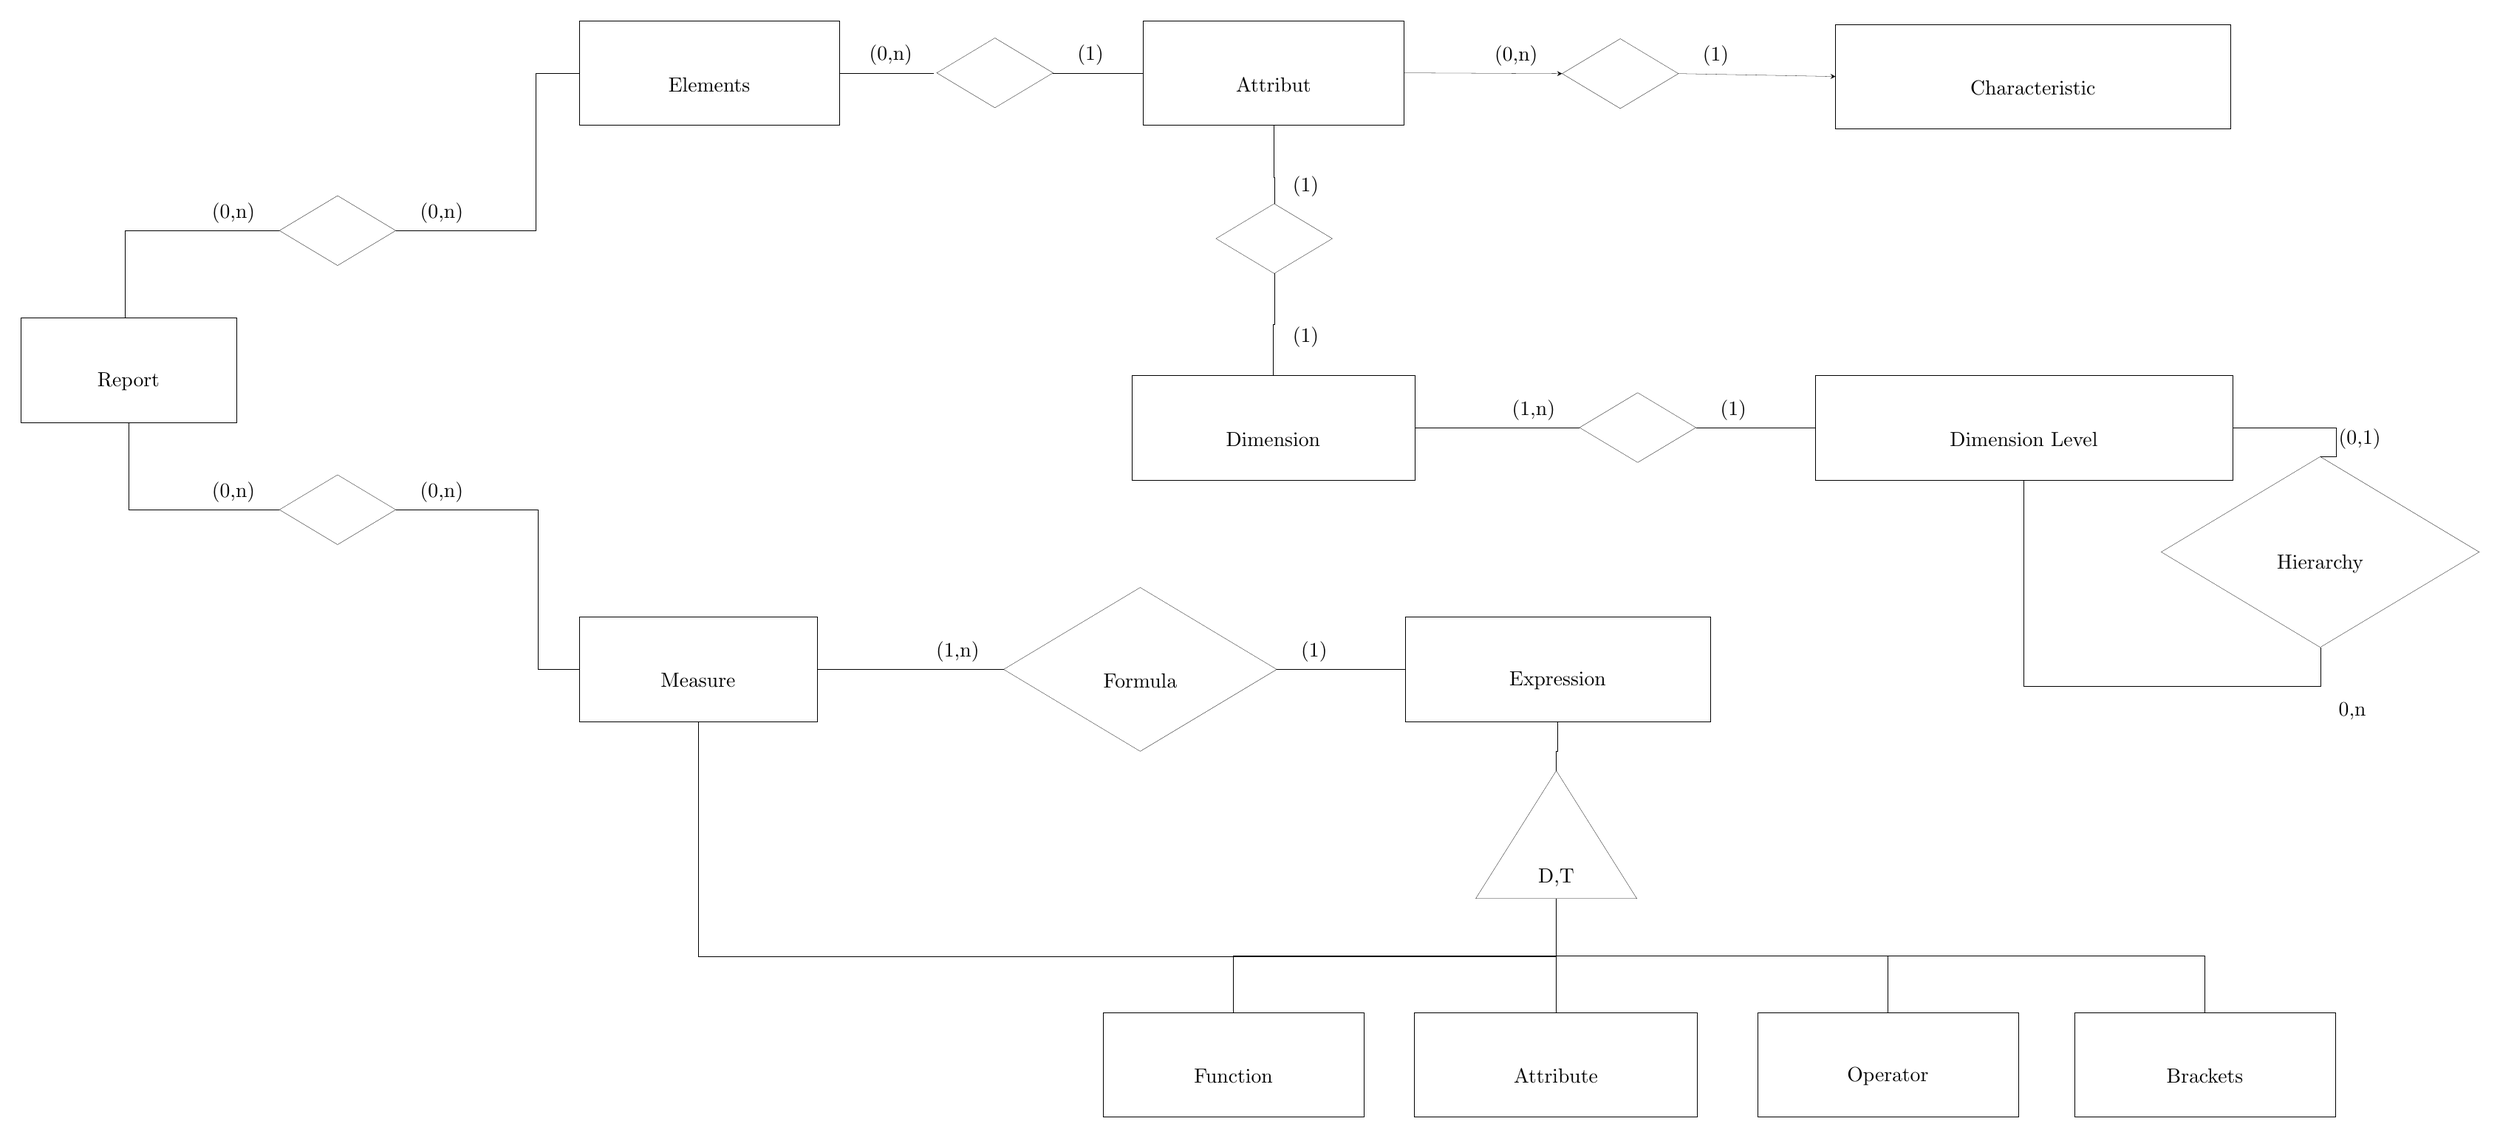
\begin{tikzpicture}
\pgftransformxscale{1.000000}
\pgftransformyscale{-1.000000}
\definecolor{dialinecolor}{rgb}{0.000000, 0.000000, 0.000000}
\pgfsetstrokecolor{dialinecolor}
\definecolor{dialinecolor}{rgb}{1.000000, 1.000000, 1.000000}
\pgfsetfillcolor{dialinecolor}
\definecolor{dialinecolor}{rgb}{1.000000, 1.000000, 1.000000}
\pgfsetfillcolor{dialinecolor}
\fill (24.900000\du,18.850000\du)--(24.900000\du,20.650000\du)--(29.765000\du,20.650000\du)--(29.765000\du,18.850000\du)--cycle;
\pgfsetlinewidth{0.100000\du}
\pgfsetdash{}{0pt}
\pgfsetmiterjoin
\definecolor{dialinecolor}{rgb}{0.000000, 0.000000, 0.000000}
\pgfsetstrokecolor{dialinecolor}
\draw (24.900000\du,18.850000\du)--(24.900000\du,20.650000\du)--(29.765000\du,20.650000\du)--(29.765000\du,18.850000\du)--cycle;
% setfont left to latex
\definecolor{dialinecolor}{rgb}{0.000000, 0.000000, 0.000000}
\pgfsetstrokecolor{dialinecolor}
\node at (27.332500\du,19.950000\du){Dimension};
\definecolor{dialinecolor}{rgb}{1.000000, 1.000000, 1.000000}
\pgfsetfillcolor{dialinecolor}
\fill (36.650000\du,18.850000\du)--(36.650000\du,20.650000\du)--(43.825000\du,20.650000\du)--(43.825000\du,18.850000\du)--cycle;
\pgfsetlinewidth{0.100000\du}
\pgfsetdash{}{0pt}
\pgfsetmiterjoin
\definecolor{dialinecolor}{rgb}{0.000000, 0.000000, 0.000000}
\pgfsetstrokecolor{dialinecolor}
\draw (36.650000\du,18.850000\du)--(36.650000\du,20.650000\du)--(43.825000\du,20.650000\du)--(43.825000\du,18.850000\du)--cycle;
% setfont left to latex
\definecolor{dialinecolor}{rgb}{0.000000, 0.000000, 0.000000}
\pgfsetstrokecolor{dialinecolor}
\node at (40.237500\du,19.950000\du){Dimension Level};
\definecolor{dialinecolor}{rgb}{1.000000, 1.000000, 1.000000}
\pgfsetfillcolor{dialinecolor}
\fill (15.400000\du,12.750000\du)--(15.400000\du,14.550000\du)--(19.880000\du,14.550000\du)--(19.880000\du,12.750000\du)--cycle;
\pgfsetlinewidth{0.100000\du}
\pgfsetdash{}{0pt}
\pgfsetmiterjoin
\definecolor{dialinecolor}{rgb}{0.000000, 0.000000, 0.000000}
\pgfsetstrokecolor{dialinecolor}
\draw (15.400000\du,12.750000\du)--(15.400000\du,14.550000\du)--(19.880000\du,14.550000\du)--(19.880000\du,12.750000\du)--cycle;
% setfont left to latex
\definecolor{dialinecolor}{rgb}{0.000000, 0.000000, 0.000000}
\pgfsetstrokecolor{dialinecolor}
\node at (17.640000\du,13.850000\du){Elements};
\definecolor{dialinecolor}{rgb}{1.000000, 1.000000, 1.000000}
\pgfsetfillcolor{dialinecolor}
\fill (25.100000\du,12.750000\du)--(25.100000\du,14.550000\du)--(29.580000\du,14.550000\du)--(29.580000\du,12.750000\du)--cycle;
\pgfsetlinewidth{0.100000\du}
\pgfsetdash{}{0pt}
\pgfsetmiterjoin
\definecolor{dialinecolor}{rgb}{0.000000, 0.000000, 0.000000}
\pgfsetstrokecolor{dialinecolor}
\draw (25.100000\du,12.750000\du)--(25.100000\du,14.550000\du)--(29.580000\du,14.550000\du)--(29.580000\du,12.750000\du)--cycle;
% setfont left to latex
\definecolor{dialinecolor}{rgb}{0.000000, 0.000000, 0.000000}
\pgfsetstrokecolor{dialinecolor}
\node at (27.340000\du,13.850000\du){Attribut};
\definecolor{dialinecolor}{rgb}{1.000000, 1.000000, 1.000000}
\pgfsetfillcolor{dialinecolor}
\fill (42.600000\du,21.889500\du)--(45.332500\du,20.250000\du)--(48.065000\du,21.889500\du)--(45.332500\du,23.529000\du)--cycle;
\pgfsetlinewidth{0.100000\du}
\pgfsetdash{}{0pt}
\pgfsetmiterjoin
\definecolor{dialinecolor}{rgb}{0.000000, 0.000000, 0.000000}
\pgfsetstrokecolor{dialinecolor}
\draw (42.600000\du,21.889500\du)--(45.332500\du,20.250000\du)--(48.065000\du,21.889500\du)--(45.332500\du,23.529000\du)--cycle;
% setfont left to latex
\definecolor{dialinecolor}{rgb}{0.000000, 0.000000, 0.000000}
\pgfsetstrokecolor{dialinecolor}
\node[anchor=west] at (45.532500\du,19.950000\du){(0,1)};
\definecolor{dialinecolor}{rgb}{0.000000, 0.000000, 0.000000}
\pgfsetstrokecolor{dialinecolor}
\node[anchor=west] at (45.532500\du,24.629000\du){0,n};
\definecolor{dialinecolor}{rgb}{0.000000, 0.000000, 0.000000}
\pgfsetstrokecolor{dialinecolor}
\node at (45.332500\du,22.089500\du){Hierarchy};
\pgfsetlinewidth{0.100000\du}
\pgfsetdash{}{0pt}
\pgfsetmiterjoin
\pgfsetbuttcap
\definecolor{dialinecolor}{rgb}{0.000000, 0.000000, 0.000000}
\pgfsetstrokecolor{dialinecolor}
\draw (40.237500\du,20.650000\du)--(40.237500\du,24.200000\du)--(45.332500\du,24.200000\du)--(45.332500\du,23.529000\du);
\pgfsetlinewidth{0.100000\du}
\pgfsetdash{}{0pt}
\pgfsetmiterjoin
\pgfsetbuttcap
\definecolor{dialinecolor}{rgb}{0.000000, 0.000000, 0.000000}
\pgfsetstrokecolor{dialinecolor}
\draw (43.825000\du,19.750000\du)--(45.600000\du,19.750000\du)--(45.600000\du,20.250000\du)--(45.332500\du,20.250000\du);
\definecolor{dialinecolor}{rgb}{1.000000, 1.000000, 1.000000}
\pgfsetfillcolor{dialinecolor}
\fill (32.600000\du,19.750000\du)--(33.600000\du,19.150000\du)--(34.600000\du,19.750000\du)--(33.600000\du,20.350000\du)--cycle;
\pgfsetlinewidth{0.100000\du}
\pgfsetdash{}{0pt}
\pgfsetmiterjoin
\definecolor{dialinecolor}{rgb}{0.000000, 0.000000, 0.000000}
\pgfsetstrokecolor{dialinecolor}
\draw (32.600000\du,19.750000\du)--(33.600000\du,19.150000\du)--(34.600000\du,19.750000\du)--(33.600000\du,20.350000\du)--cycle;
% setfont left to latex
\definecolor{dialinecolor}{rgb}{0.000000, 0.000000, 0.000000}
\pgfsetstrokecolor{dialinecolor}
\node[anchor=east] at (32.300000\du,19.450000\du){(1,n) };
\definecolor{dialinecolor}{rgb}{0.000000, 0.000000, 0.000000}
\pgfsetstrokecolor{dialinecolor}
\node[anchor=west] at (34.900000\du,19.450000\du){(1) };
\definecolor{dialinecolor}{rgb}{0.000000, 0.000000, 0.000000}
\pgfsetstrokecolor{dialinecolor}
\node at (33.600000\du,19.950000\du){};
\pgfsetlinewidth{0.100000\du}
\pgfsetdash{}{0pt}
\pgfsetmiterjoin
\pgfsetbuttcap
\definecolor{dialinecolor}{rgb}{0.000000, 0.000000, 0.000000}
\pgfsetstrokecolor{dialinecolor}
\draw (29.765000\du,19.750000\du)--(29.815000\du,19.750000\du)--(32.550000\du,19.750000\du)--(32.600000\du,19.750000\du);
\pgfsetlinewidth{0.100000\du}
\pgfsetdash{}{0pt}
\pgfsetmiterjoin
\pgfsetbuttcap
\definecolor{dialinecolor}{rgb}{0.000000, 0.000000, 0.000000}
\pgfsetstrokecolor{dialinecolor}
\draw (34.600000\du,19.750000\du)--(34.650000\du,19.750000\du)--(36.600000\du,19.750000\du)--(36.650000\du,19.750000\du);
\definecolor{dialinecolor}{rgb}{1.000000, 1.000000, 1.000000}
\pgfsetfillcolor{dialinecolor}
\fill (21.550000\du,13.650000\du)--(22.550000\du,13.050000\du)--(23.550000\du,13.650000\du)--(22.550000\du,14.250000\du)--cycle;
\pgfsetlinewidth{0.100000\du}
\pgfsetdash{}{0pt}
\pgfsetmiterjoin
\definecolor{dialinecolor}{rgb}{0.000000, 0.000000, 0.000000}
\pgfsetstrokecolor{dialinecolor}
\draw (21.550000\du,13.650000\du)--(22.550000\du,13.050000\du)--(23.550000\du,13.650000\du)--(22.550000\du,14.250000\du)--cycle;
% setfont left to latex
\definecolor{dialinecolor}{rgb}{0.000000, 0.000000, 0.000000}
\pgfsetstrokecolor{dialinecolor}
\node[anchor=east] at (21.250000\du,13.350000\du){(0,n)};
\definecolor{dialinecolor}{rgb}{0.000000, 0.000000, 0.000000}
\pgfsetstrokecolor{dialinecolor}
\node[anchor=west] at (23.850000\du,13.350000\du){(1)};
\definecolor{dialinecolor}{rgb}{0.000000, 0.000000, 0.000000}
\pgfsetstrokecolor{dialinecolor}
\node at (22.550000\du,13.850000\du){};
\pgfsetlinewidth{0.100000\du}
\pgfsetdash{}{0pt}
\pgfsetmiterjoin
\pgfsetbuttcap
\definecolor{dialinecolor}{rgb}{0.000000, 0.000000, 0.000000}
\pgfsetstrokecolor{dialinecolor}
\draw (19.880000\du,13.650000\du)--(19.930000\du,13.650000\du)--(21.450177\du,13.650000\du)--(21.500177\du,13.650000\du);
\pgfsetlinewidth{0.100000\du}
\pgfsetdash{}{0pt}
\pgfsetmiterjoin
\pgfsetbuttcap
\definecolor{dialinecolor}{rgb}{0.000000, 0.000000, 0.000000}
\pgfsetstrokecolor{dialinecolor}
\draw (23.550000\du,13.650000\du)--(23.600000\du,13.650000\du)--(25.050000\du,13.650000\du)--(25.100000\du,13.650000\du);
\pgfsetlinewidth{0.100000\du}
\pgfsetdash{}{0pt}
\pgfsetmiterjoin
\pgfsetbuttcap
\definecolor{dialinecolor}{rgb}{0.000000, 0.000000, 0.000000}
\pgfsetstrokecolor{dialinecolor}
\draw (27.340000\du,14.550000\du)--(27.340000\du,15.450000\du)--(27.350000\du,15.450000\du)--(27.350000\du,15.900000\du);
\definecolor{dialinecolor}{rgb}{1.000000, 1.000000, 1.000000}
\pgfsetfillcolor{dialinecolor}
\fill (26.350000\du,16.500000\du)--(27.350000\du,15.900000\du)--(28.350000\du,16.500000\du)--(27.350000\du,17.100000\du)--cycle;
\pgfsetlinewidth{0.100000\du}
\pgfsetdash{}{0pt}
\pgfsetmiterjoin
\definecolor{dialinecolor}{rgb}{0.000000, 0.000000, 0.000000}
\pgfsetstrokecolor{dialinecolor}
\draw (26.350000\du,16.500000\du)--(27.350000\du,15.900000\du)--(28.350000\du,16.500000\du)--(27.350000\du,17.100000\du)--cycle;
% setfont left to latex
\definecolor{dialinecolor}{rgb}{0.000000, 0.000000, 0.000000}
\pgfsetstrokecolor{dialinecolor}
\node[anchor=west] at (27.550000\du,15.600000\du){(1)};
\definecolor{dialinecolor}{rgb}{0.000000, 0.000000, 0.000000}
\pgfsetstrokecolor{dialinecolor}
\node[anchor=west] at (27.550000\du,18.200000\du){(1)};
\definecolor{dialinecolor}{rgb}{0.000000, 0.000000, 0.000000}
\pgfsetstrokecolor{dialinecolor}
\node at (27.350000\du,16.700000\du){};
\pgfsetlinewidth{0.100000\du}
\pgfsetdash{}{0pt}
\pgfsetmiterjoin
\pgfsetbuttcap
\definecolor{dialinecolor}{rgb}{0.000000, 0.000000, 0.000000}
\pgfsetstrokecolor{dialinecolor}
\draw (27.350000\du,17.100000\du)--(27.350000\du,17.975000\du)--(27.332500\du,17.975000\du)--(27.332500\du,18.850000\du);
\definecolor{dialinecolor}{rgb}{1.000000, 1.000000, 1.000000}
\pgfsetfillcolor{dialinecolor}
\fill (15.400000\du,23.000000\du)--(15.400000\du,24.800000\du)--(19.495000\du,24.800000\du)--(19.495000\du,23.000000\du)--cycle;
\pgfsetlinewidth{0.100000\du}
\pgfsetdash{}{0pt}
\pgfsetmiterjoin
\definecolor{dialinecolor}{rgb}{0.000000, 0.000000, 0.000000}
\pgfsetstrokecolor{dialinecolor}
\draw (15.400000\du,23.000000\du)--(15.400000\du,24.800000\du)--(19.495000\du,24.800000\du)--(19.495000\du,23.000000\du)--cycle;
% setfont left to latex
\definecolor{dialinecolor}{rgb}{0.000000, 0.000000, 0.000000}
\pgfsetstrokecolor{dialinecolor}
\node at (17.447500\du,24.100000\du){Measure};
\definecolor{dialinecolor}{rgb}{1.000000, 1.000000, 1.000000}
\pgfsetfillcolor{dialinecolor}
\fill (29.600000\du,23.000000\du)--(29.600000\du,24.800000\du)--(34.850000\du,24.800000\du)--(34.850000\du,23.000000\du)--cycle;
\pgfsetlinewidth{0.100000\du}
\pgfsetdash{}{0pt}
\pgfsetmiterjoin
\definecolor{dialinecolor}{rgb}{0.000000, 0.000000, 0.000000}
\pgfsetstrokecolor{dialinecolor}
\draw (29.600000\du,23.000000\du)--(29.600000\du,24.800000\du)--(34.850000\du,24.800000\du)--(34.850000\du,23.000000\du)--cycle;
% setfont left to latex
\definecolor{dialinecolor}{rgb}{0.000000, 0.000000, 0.000000}
\pgfsetstrokecolor{dialinecolor}
\node at (32.225000\du,24.100000\du){Expression};
\definecolor{dialinecolor}{rgb}{1.000000, 1.000000, 1.000000}
\pgfsetfillcolor{dialinecolor}
\fill (22.700000\du,23.908500\du)--(25.047500\du,22.500000\du)--(27.395000\du,23.908500\du)--(25.047500\du,25.317000\du)--cycle;
\pgfsetlinewidth{0.100000\du}
\pgfsetdash{}{0pt}
\pgfsetmiterjoin
\definecolor{dialinecolor}{rgb}{0.000000, 0.000000, 0.000000}
\pgfsetstrokecolor{dialinecolor}
\draw (22.700000\du,23.908500\du)--(25.047500\du,22.500000\du)--(27.395000\du,23.908500\du)--(25.047500\du,25.317000\du)--cycle;
% setfont left to latex
\definecolor{dialinecolor}{rgb}{0.000000, 0.000000, 0.000000}
\pgfsetstrokecolor{dialinecolor}
\node[anchor=east] at (22.400000\du,23.608500\du){(1,n)};
\definecolor{dialinecolor}{rgb}{0.000000, 0.000000, 0.000000}
\pgfsetstrokecolor{dialinecolor}
\node[anchor=west] at (27.695000\du,23.608500\du){(1)};
\definecolor{dialinecolor}{rgb}{0.000000, 0.000000, 0.000000}
\pgfsetstrokecolor{dialinecolor}
\node at (25.047500\du,24.108500\du){Formula};
\pgfsetlinewidth{0.100000\du}
\pgfsetdash{}{0pt}
\pgfsetmiterjoin
\pgfsetbuttcap
\definecolor{dialinecolor}{rgb}{0.000000, 0.000000, 0.000000}
\pgfsetstrokecolor{dialinecolor}
\draw (19.495000\du,23.900000\du)--(21.097500\du,23.900000\du)--(21.097500\du,23.908500\du)--(22.700000\du,23.908500\du);
\pgfsetlinewidth{0.100000\du}
\pgfsetdash{}{0pt}
\pgfsetmiterjoin
\pgfsetbuttcap
\definecolor{dialinecolor}{rgb}{0.000000, 0.000000, 0.000000}
\pgfsetstrokecolor{dialinecolor}
\draw (27.395000\du,23.908500\du)--(28.497500\du,23.908500\du)--(28.497500\du,23.900000\du)--(29.600000\du,23.900000\du);
\pgfsetlinewidth{0.100000\du}
\pgfsetdash{}{0pt}
\pgfsetdash{}{0pt}
\pgfsetbuttcap
\pgfsetmiterjoin
\pgfsetlinewidth{0.100000\du}
\pgfsetbuttcap
\pgfsetmiterjoin
\pgfsetdash{}{0pt}
\definecolor{dialinecolor}{rgb}{1.000000, 1.000000, 1.000000}
\pgfsetfillcolor{dialinecolor}
\fill (30.815000\du,27.850000\du)--(33.585000\du,27.850000\du)--(32.200000\du,25.650000\du)--cycle;
\definecolor{dialinecolor}{rgb}{0.000000, 0.000000, 0.000000}
\pgfsetstrokecolor{dialinecolor}
\draw (30.815000\du,27.850000\du)--(33.585000\du,27.850000\du)--(32.200000\du,25.650000\du)--cycle;
% setfont left to latex
\definecolor{dialinecolor}{rgb}{0.000000, 0.000000, 0.000000}
\pgfsetstrokecolor{dialinecolor}
\node at (32.200000\du,27.500000\du){D,T};
\pgfsetlinewidth{0.100000\du}
\pgfsetdash{}{0pt}
\pgfsetmiterjoin
\pgfsetbuttcap
\definecolor{dialinecolor}{rgb}{0.000000, 0.000000, 0.000000}
\pgfsetstrokecolor{dialinecolor}
\draw (32.225000\du,24.800000\du)--(32.225000\du,25.312500\du)--(32.200000\du,25.312500\du)--(32.200000\du,25.650000\du);
\definecolor{dialinecolor}{rgb}{1.000000, 1.000000, 1.000000}
\pgfsetfillcolor{dialinecolor}
\fill (24.410000\du,29.805000\du)--(24.410000\du,31.605000\du)--(28.890000\du,31.605000\du)--(28.890000\du,29.805000\du)--cycle;
\pgfsetlinewidth{0.100000\du}
\pgfsetdash{}{0pt}
\pgfsetmiterjoin
\definecolor{dialinecolor}{rgb}{0.000000, 0.000000, 0.000000}
\pgfsetstrokecolor{dialinecolor}
\draw (24.410000\du,29.805000\du)--(24.410000\du,31.605000\du)--(28.890000\du,31.605000\du)--(28.890000\du,29.805000\du)--cycle;
% setfont left to latex
\definecolor{dialinecolor}{rgb}{0.000000, 0.000000, 0.000000}
\pgfsetstrokecolor{dialinecolor}
\node at (26.650000\du,30.905000\du){Function};
\definecolor{dialinecolor}{rgb}{1.000000, 1.000000, 1.000000}
\pgfsetfillcolor{dialinecolor}
\fill (29.760000\du,29.805000\du)--(29.760000\du,31.605000\du)--(34.625000\du,31.605000\du)--(34.625000\du,29.805000\du)--cycle;
\pgfsetlinewidth{0.100000\du}
\pgfsetdash{}{0pt}
\pgfsetmiterjoin
\definecolor{dialinecolor}{rgb}{0.000000, 0.000000, 0.000000}
\pgfsetstrokecolor{dialinecolor}
\draw (29.760000\du,29.805000\du)--(29.760000\du,31.605000\du)--(34.625000\du,31.605000\du)--(34.625000\du,29.805000\du)--cycle;
% setfont left to latex
\definecolor{dialinecolor}{rgb}{0.000000, 0.000000, 0.000000}
\pgfsetstrokecolor{dialinecolor}
\node at (32.192500\du,30.905000\du){Attribute};
\definecolor{dialinecolor}{rgb}{1.000000, 1.000000, 1.000000}
\pgfsetfillcolor{dialinecolor}
\fill (35.660000\du,29.805000\du)--(35.660000\du,31.605000\du)--(40.140000\du,31.605000\du)--(40.140000\du,29.805000\du)--cycle;
\pgfsetlinewidth{0.100000\du}
\pgfsetdash{}{0pt}
\pgfsetmiterjoin
\definecolor{dialinecolor}{rgb}{0.000000, 0.000000, 0.000000}
\pgfsetstrokecolor{dialinecolor}
\draw (35.660000\du,29.805000\du)--(35.660000\du,31.605000\du)--(40.140000\du,31.605000\du)--(40.140000\du,29.805000\du)--cycle;
% setfont left to latex
\definecolor{dialinecolor}{rgb}{0.000000, 0.000000, 0.000000}
\pgfsetstrokecolor{dialinecolor}
\node at (37.900000\du,30.905000\du){Operator};
\definecolor{dialinecolor}{rgb}{1.000000, 1.000000, 1.000000}
\pgfsetfillcolor{dialinecolor}
\fill (41.110000\du,29.805000\du)--(41.110000\du,31.605000\du)--(45.590000\du,31.605000\du)--(45.590000\du,29.805000\du)--cycle;
\pgfsetlinewidth{0.100000\du}
\pgfsetdash{}{0pt}
\pgfsetmiterjoin
\definecolor{dialinecolor}{rgb}{0.000000, 0.000000, 0.000000}
\pgfsetstrokecolor{dialinecolor}
\draw (41.110000\du,29.805000\du)--(41.110000\du,31.605000\du)--(45.590000\du,31.605000\du)--(45.590000\du,29.805000\du)--cycle;
% setfont left to latex
\definecolor{dialinecolor}{rgb}{0.000000, 0.000000, 0.000000}
\pgfsetstrokecolor{dialinecolor}
\node at (43.350000\du,30.905000\du){Brackets};
\pgfsetlinewidth{0.100000\du}
\pgfsetdash{}{0pt}
\pgfsetmiterjoin
\pgfsetbuttcap
\definecolor{dialinecolor}{rgb}{0.000000, 0.000000, 0.000000}
\pgfsetstrokecolor{dialinecolor}
\draw (32.200000\du,27.850000\du)--(32.200000\du,28.827500\du)--(32.192500\du,28.827500\du)--(32.192500\du,29.805000\du);
\pgfsetlinewidth{0.100000\du}
\pgfsetdash{}{0pt}
\pgfsetmiterjoin
\pgfsetbuttcap
\definecolor{dialinecolor}{rgb}{0.000000, 0.000000, 0.000000}
\pgfsetstrokecolor{dialinecolor}
\draw (32.200000\du,27.850000\du)--(32.200000\du,28.827500\du)--(37.900000\du,28.827500\du)--(37.900000\du,29.805000\du);
\pgfsetlinewidth{0.100000\du}
\pgfsetdash{}{0pt}
\pgfsetmiterjoin
\pgfsetbuttcap
\definecolor{dialinecolor}{rgb}{0.000000, 0.000000, 0.000000}
\pgfsetstrokecolor{dialinecolor}
\draw (32.200000\du,27.850000\du)--(32.200000\du,28.827500\du)--(26.650000\du,28.827500\du)--(26.650000\du,29.805000\du);
\pgfsetlinewidth{0.100000\du}
\pgfsetdash{}{0pt}
\pgfsetmiterjoin
\pgfsetbuttcap
\definecolor{dialinecolor}{rgb}{0.000000, 0.000000, 0.000000}
\pgfsetstrokecolor{dialinecolor}
\draw (32.200000\du,27.850000\du)--(32.200000\du,28.850000\du)--(17.447500\du,28.850000\du)--(17.447500\du,24.800000\du);
\pgfsetlinewidth{0.100000\du}
\pgfsetdash{}{0pt}
\pgfsetmiterjoin
\pgfsetbuttcap
\definecolor{dialinecolor}{rgb}{0.000000, 0.000000, 0.000000}
\pgfsetstrokecolor{dialinecolor}
\draw (32.200000\du,27.850000\du)--(32.200000\du,28.827500\du)--(43.350000\du,28.827500\du)--(43.350000\du,29.805000\du);
\definecolor{dialinecolor}{rgb}{1.000000, 1.000000, 1.000000}
\pgfsetfillcolor{dialinecolor}
\fill (5.800000\du,17.862500\du)--(5.800000\du,19.662500\du)--(9.510000\du,19.662500\du)--(9.510000\du,17.862500\du)--cycle;
\pgfsetlinewidth{0.100000\du}
\pgfsetdash{}{0pt}
\pgfsetmiterjoin
\definecolor{dialinecolor}{rgb}{0.000000, 0.000000, 0.000000}
\pgfsetstrokecolor{dialinecolor}
\draw (5.800000\du,17.862500\du)--(5.800000\du,19.662500\du)--(9.510000\du,19.662500\du)--(9.510000\du,17.862500\du)--cycle;
% setfont left to latex
\definecolor{dialinecolor}{rgb}{0.000000, 0.000000, 0.000000}
\pgfsetstrokecolor{dialinecolor}
\node at (7.655000\du,18.962500\du){Report};
\definecolor{dialinecolor}{rgb}{1.000000, 1.000000, 1.000000}
\pgfsetfillcolor{dialinecolor}
\fill (10.250000\du,16.362500\du)--(11.250000\du,15.762500\du)--(12.250000\du,16.362500\du)--(11.250000\du,16.962500\du)--cycle;
\pgfsetlinewidth{0.100000\du}
\pgfsetdash{}{0pt}
\pgfsetmiterjoin
\definecolor{dialinecolor}{rgb}{0.000000, 0.000000, 0.000000}
\pgfsetstrokecolor{dialinecolor}
\draw (10.250000\du,16.362500\du)--(11.250000\du,15.762500\du)--(12.250000\du,16.362500\du)--(11.250000\du,16.962500\du)--cycle;
% setfont left to latex
\definecolor{dialinecolor}{rgb}{0.000000, 0.000000, 0.000000}
\pgfsetstrokecolor{dialinecolor}
\node[anchor=east] at (9.950000\du,16.062500\du){(0,n)};
\definecolor{dialinecolor}{rgb}{0.000000, 0.000000, 0.000000}
\pgfsetstrokecolor{dialinecolor}
\node[anchor=west] at (12.550000\du,16.062500\du){(0,n)};
\definecolor{dialinecolor}{rgb}{0.000000, 0.000000, 0.000000}
\pgfsetstrokecolor{dialinecolor}
\node at (11.250000\du,16.562500\du){};
\pgfsetlinewidth{0.100000\du}
\pgfsetdash{}{0pt}
\pgfsetmiterjoin
\pgfsetbuttcap
\definecolor{dialinecolor}{rgb}{0.000000, 0.000000, 0.000000}
\pgfsetstrokecolor{dialinecolor}
\draw (7.655000\du,17.862500\du)--(7.600000\du,17.862500\du)--(7.600000\du,16.362500\du)--(10.250000\du,16.362500\du);
\pgfsetlinewidth{0.100000\du}
\pgfsetdash{}{0pt}
\pgfsetmiterjoin
\pgfsetbuttcap
\definecolor{dialinecolor}{rgb}{0.000000, 0.000000, 0.000000}
\pgfsetstrokecolor{dialinecolor}
\draw (12.250000\du,16.362500\du)--(14.650000\du,16.362500\du)--(14.650000\du,13.650000\du)--(15.400000\du,13.650000\du);
\definecolor{dialinecolor}{rgb}{1.000000, 1.000000, 1.000000}
\pgfsetfillcolor{dialinecolor}
\fill (10.250000\du,21.162500\du)--(11.250000\du,20.562500\du)--(12.250000\du,21.162500\du)--(11.250000\du,21.762500\du)--cycle;
\pgfsetlinewidth{0.100000\du}
\pgfsetdash{}{0pt}
\pgfsetmiterjoin
\definecolor{dialinecolor}{rgb}{0.000000, 0.000000, 0.000000}
\pgfsetstrokecolor{dialinecolor}
\draw (10.250000\du,21.162500\du)--(11.250000\du,20.562500\du)--(12.250000\du,21.162500\du)--(11.250000\du,21.762500\du)--cycle;
% setfont left to latex
\definecolor{dialinecolor}{rgb}{0.000000, 0.000000, 0.000000}
\pgfsetstrokecolor{dialinecolor}
\node[anchor=east] at (9.950000\du,20.862500\du){(0,n)};
\definecolor{dialinecolor}{rgb}{0.000000, 0.000000, 0.000000}
\pgfsetstrokecolor{dialinecolor}
\node[anchor=west] at (12.550000\du,20.862500\du){(0,n)};
\definecolor{dialinecolor}{rgb}{0.000000, 0.000000, 0.000000}
\pgfsetstrokecolor{dialinecolor}
\node at (11.250000\du,21.362500\du){};
\pgfsetlinewidth{0.100000\du}
\pgfsetdash{}{0pt}
\pgfsetmiterjoin
\pgfsetbuttcap
\definecolor{dialinecolor}{rgb}{0.000000, 0.000000, 0.000000}
\pgfsetstrokecolor{dialinecolor}
\draw (7.655000\du,19.662500\du)--(7.655000\du,21.162500\du)--(10.250000\du,21.162500\du);
\pgfsetlinewidth{0.100000\du}
\pgfsetdash{}{0pt}
\pgfsetmiterjoin
\pgfsetbuttcap
\definecolor{dialinecolor}{rgb}{0.000000, 0.000000, 0.000000}
\pgfsetstrokecolor{dialinecolor}
\draw (12.250000\du,21.162500\du)--(14.700000\du,21.162500\du)--(14.700000\du,23.900000\du)--(15.400000\du,23.900000\du);
\definecolor{dialinecolor}{rgb}{1.000000, 1.000000, 1.000000}
\pgfsetfillcolor{dialinecolor}
\fill (37.000000\du,12.812500\du)--(37.000000\du,14.612500\du)--(43.790000\du,14.612500\du)--(43.790000\du,12.812500\du)--cycle;
\pgfsetlinewidth{0.100000\du}
\pgfsetdash{}{0pt}
\pgfsetmiterjoin
\definecolor{dialinecolor}{rgb}{0.000000, 0.000000, 0.000000}
\pgfsetstrokecolor{dialinecolor}
\draw (37.000000\du,12.812500\du)--(37.000000\du,14.612500\du)--(43.790000\du,14.612500\du)--(43.790000\du,12.812500\du)--cycle;
% setfont left to latex
\definecolor{dialinecolor}{rgb}{0.000000, 0.000000, 0.000000}
\pgfsetstrokecolor{dialinecolor}
\node at (40.395000\du,13.912500\du){Characteristic};
\definecolor{dialinecolor}{rgb}{1.000000, 1.000000, 1.000000}
\pgfsetfillcolor{dialinecolor}
\fill (32.300000\du,13.662500\du)--(33.300000\du,13.062500\du)--(34.300000\du,13.662500\du)--(33.300000\du,14.262500\du)--cycle;
\pgfsetlinewidth{0.100000\du}
\pgfsetdash{}{0pt}
\pgfsetmiterjoin
\definecolor{dialinecolor}{rgb}{0.000000, 0.000000, 0.000000}
\pgfsetstrokecolor{dialinecolor}
\draw (32.300000\du,13.662500\du)--(33.300000\du,13.062500\du)--(34.300000\du,13.662500\du)--(33.300000\du,14.262500\du)--cycle;
% setfont left to latex
\definecolor{dialinecolor}{rgb}{0.000000, 0.000000, 0.000000}
\pgfsetstrokecolor{dialinecolor}
\node[anchor=east] at (32.000000\du,13.362500\du){(0,n)};
\definecolor{dialinecolor}{rgb}{0.000000, 0.000000, 0.000000}
\pgfsetstrokecolor{dialinecolor}
\node[anchor=west] at (34.600000\du,13.362500\du){(1)};
\definecolor{dialinecolor}{rgb}{0.000000, 0.000000, 0.000000}
\pgfsetstrokecolor{dialinecolor}
\node at (33.300000\du,13.862500\du){};
\pgfsetlinewidth{0.100000\du}
\pgfsetdash{}{0pt}
\pgfsetdash{}{0pt}
\pgfsetbuttcap
{
\definecolor{dialinecolor}{rgb}{0.000000, 0.000000, 0.000000}
\pgfsetfillcolor{dialinecolor}
% was here!!!
\pgfsetarrowsend{stealth}
\definecolor{dialinecolor}{rgb}{0.000000, 0.000000, 0.000000}
\pgfsetstrokecolor{dialinecolor}
\draw (29.580000\du,13.650000\du)--(32.300000\du,13.662500\du);
}
\pgfsetlinewidth{0.100000\du}
\pgfsetdash{}{0pt}
\pgfsetdash{}{0pt}
\pgfsetbuttcap
{
\definecolor{dialinecolor}{rgb}{0.000000, 0.000000, 0.000000}
\pgfsetfillcolor{dialinecolor}
% was here!!!
\pgfsetarrowsend{stealth}
\definecolor{dialinecolor}{rgb}{0.000000, 0.000000, 0.000000}
\pgfsetstrokecolor{dialinecolor}
\draw (34.300000\du,13.662500\du)--(37.000000\du,13.712500\du);
}
\end{tikzpicture}
}
  \end{figure}

  \subsection{Geschäftsobjekte}
  Der Begriff Geschäftsobjekt wird aus dem \textit{DataRocket}-Vokabular
  übernommen. Geschäftsobjekte sind Datenobjekte innerhalb eines Unternehmens,
  welche isoliert betrachtet werden können. Sie können sowohl der Klasse der
  Transaktionsdaten als auch der Stammdaten angehören. Sie bilden den zentralen
  Baustein der \textit{DataRocket}-Software. Ein Geschäftsobjekt kann zum
  Beispiel das \textit{Produkt} aber auch die \textit{Umsatztransaktion} sein.
  Das Geschäftsobjekt kann mit dem Bezugsobjekt der \textit{H2 for
  Reporting}-Sprache verglichen werden. \todo{Wo liegen die Ähnlichkeiten?}

  \begin{figure}[caption={Teilsprache---Geschäftsobjekt}, label={geschaeftsobjekt}]
    \resizebox{200px}{!}{% Graphic for TeX using PGF
% Title: /home/indenml/code/bachelor_thesis/content/figures/language_spec-erm-geschaeftsobjekt.dia
% Creator: Dia v0.97.3
% CreationDate: Sun Aug  7 23:24:42 2016
% For: indenml
% \usepackage{tikz}
% The following commands are not supported in PSTricks at present
% We define them conditionally, so when they are implemented,
% this pgf file will use them.
\ifx\du\undefined{}
  \newlength{\du}
\fi
\setlength{\du}{15\unitlength}
\begin{tikzpicture}
\pgftransformxscale{1.000000}
\pgftransformyscale{-1.000000}
\definecolor{dialinecolor}{rgb}{0.000000, 0.000000, 0.000000}
\pgfsetstrokecolor{dialinecolor}
\definecolor{dialinecolor}{rgb}{1.000000, 1.000000, 1.000000}
\pgfsetfillcolor{dialinecolor}
\definecolor{dialinecolor}{rgb}{1.000000, 1.000000, 1.000000}
\pgfsetfillcolor{dialinecolor}
\fill (30.495000\du,7.625000\du)--(30.495000\du,9.425000\du)--(34.975000\du,9.425000\du)--(34.975000\du,7.625000\du)--cycle;
\pgfsetlinewidth{0.100000\du}
\pgfsetdash{}{0pt}
\pgfsetmiterjoin
\definecolor{dialinecolor}{rgb}{0.000000, 0.000000, 0.000000}
\pgfsetstrokecolor{dialinecolor}
\draw (30.495000\du,7.625000\du)--(30.495000\du,9.425000\du)--(34.975000\du,9.425000\du)--(34.975000\du,7.625000\du)--cycle;
% setfont left to latex
\definecolor{dialinecolor}{rgb}{0.000000, 0.000000, 0.000000}
\pgfsetstrokecolor{dialinecolor}
\node at (32.735000\du,8.725000\du){Attribut};
\definecolor{dialinecolor}{rgb}{1.000000, 1.000000, 1.000000}
\pgfsetfillcolor{dialinecolor}
\fill (20.045000\du,1.537500\du)--(20.045000\du,3.337500\du)--(25.295000\du,3.337500\du)--(25.295000\du,1.537500\du)--cycle;
\pgfsetlinewidth{0.100000\du}
\pgfsetdash{}{0pt}
\pgfsetmiterjoin
\definecolor{dialinecolor}{rgb}{0.000000, 0.000000, 0.000000}
\pgfsetstrokecolor{dialinecolor}
\draw (20.045000\du,1.537500\du)--(20.045000\du,3.337500\du)--(25.295000\du,3.337500\du)--(25.295000\du,1.537500\du)--cycle;
% setfont left to latex
\definecolor{dialinecolor}{rgb}{0.000000, 0.000000, 0.000000}
\pgfsetstrokecolor{dialinecolor}
\node at (22.670000\du,2.637500\du){Ausprägung};
\definecolor{dialinecolor}{rgb}{1.000000, 1.000000, 1.000000}
\pgfsetfillcolor{dialinecolor}
\fill (30.345000\du,1.475000\du)--(30.345000\du,3.275000\du)--(37.520000\du,3.275000\du)--(37.520000\du,1.475000\du)--cycle;
\pgfsetlinewidth{0.100000\du}
\pgfsetdash{}{0pt}
\pgfsetmiterjoin
\definecolor{dialinecolor}{rgb}{0.000000, 0.000000, 0.000000}
\pgfsetstrokecolor{dialinecolor}
\draw (30.345000\du,1.475000\du)--(30.345000\du,3.275000\du)--(37.520000\du,3.275000\du)--(37.520000\du,1.475000\du)--cycle;
% setfont left to latex
\definecolor{dialinecolor}{rgb}{0.000000, 0.000000, 0.000000}
\pgfsetstrokecolor{dialinecolor}
\node at (33.932500\du,2.575000\du){Geschäftsobjekt};
\definecolor{dialinecolor}{rgb}{1.000000, 1.000000, 1.000000}
\pgfsetfillcolor{dialinecolor}
\fill (32.945000\du,5.325000\du)--(33.945000\du,4.725000\du)--(34.945000\du,5.325000\du)--(33.945000\du,5.925000\du)--cycle;
\pgfsetlinewidth{0.100000\du}
\pgfsetdash{}{0pt}
\pgfsetmiterjoin
\definecolor{dialinecolor}{rgb}{0.000000, 0.000000, 0.000000}
\pgfsetstrokecolor{dialinecolor}
\draw (32.945000\du,5.325000\du)--(33.945000\du,4.725000\du)--(34.945000\du,5.325000\du)--(33.945000\du,5.925000\du)--cycle;
% setfont left to latex
\definecolor{dialinecolor}{rgb}{0.000000, 0.000000, 0.000000}
\pgfsetstrokecolor{dialinecolor}
\node[anchor=west] at (34.145000\du,4.425000\du){(0,n)};
\definecolor{dialinecolor}{rgb}{0.000000, 0.000000, 0.000000}
\pgfsetstrokecolor{dialinecolor}
\node[anchor=west] at (34.145000\du,7.025000\du){(0,1)};
\definecolor{dialinecolor}{rgb}{0.000000, 0.000000, 0.000000}
\pgfsetstrokecolor{dialinecolor}
\node at (33.945000\du,5.525000\du){};
\pgfsetlinewidth{0.100000\du}
\pgfsetdash{}{0pt}
\pgfsetmiterjoin
\pgfsetbuttcap
\definecolor{dialinecolor}{rgb}{0.000000, 0.000000, 0.000000}
\pgfsetstrokecolor{dialinecolor}
\draw (32.735000\du,7.625000\du)--(32.735000\du,7.625000\du)--(33.945000\du,7.625000\du)--(33.945000\du,5.925000\du);
\pgfsetlinewidth{0.100000\du}
\pgfsetdash{}{0pt}
\pgfsetmiterjoin
\pgfsetbuttcap
\definecolor{dialinecolor}{rgb}{0.000000, 0.000000, 0.000000}
\pgfsetstrokecolor{dialinecolor}
\draw (33.945000\du,4.725000\du)--(33.945000\du,4.025232\du)--(33.932500\du,4.025232\du)--(33.932500\du,3.325464\du);
\definecolor{dialinecolor}{rgb}{1.000000, 1.000000, 1.000000}
\pgfsetfillcolor{dialinecolor}
\fill (28.795000\du,5.625000\du)--(29.795000\du,5.025000\du)--(30.795000\du,5.625000\du)--(29.795000\du,6.225000\du)--cycle;
\pgfsetlinewidth{0.100000\du}
\pgfsetdash{}{0pt}
\pgfsetmiterjoin
\definecolor{dialinecolor}{rgb}{0.000000, 0.000000, 0.000000}
\pgfsetstrokecolor{dialinecolor}
\draw (28.795000\du,5.625000\du)--(29.795000\du,5.025000\du)--(30.795000\du,5.625000\du)--(29.795000\du,6.225000\du)--cycle;
% setfont left to latex
\definecolor{dialinecolor}{rgb}{0.000000, 0.000000, 0.000000}
\pgfsetstrokecolor{dialinecolor}
\node[anchor=east] at (28.495000\du,5.325000\du){(0,1)};
\definecolor{dialinecolor}{rgb}{0.000000, 0.000000, 0.000000}
\pgfsetstrokecolor{dialinecolor}
\node[anchor=west] at (31.095000\du,5.325000\du){(0,n)};
\definecolor{dialinecolor}{rgb}{0.000000, 0.000000, 0.000000}
\pgfsetstrokecolor{dialinecolor}
\node at (29.795000\du,5.825000\du){};
\pgfsetlinewidth{0.100000\du}
\pgfsetdash{}{0pt}
\pgfsetmiterjoin
\pgfsetbuttcap
\definecolor{dialinecolor}{rgb}{0.000000, 0.000000, 0.000000}
\pgfsetstrokecolor{dialinecolor}
\draw (25.295000\du,2.437500\du)--(26.395000\du,2.437500\du)--(26.395000\du,5.625000\du)--(28.795000\du,5.625000\du);
\pgfsetlinewidth{0.100000\du}
\pgfsetdash{}{0pt}
\pgfsetmiterjoin
\pgfsetbuttcap
\definecolor{dialinecolor}{rgb}{0.000000, 0.000000, 0.000000}
\pgfsetstrokecolor{dialinecolor}
\draw (30.795000\du,5.625000\du)--(30.795000\du,5.675000\du)--(32.735000\du,5.675000\du)--(32.735000\du,7.625000\du);
\end{tikzpicture}
}
  \end{figure}

  Einem Geschäftsobjekt werden Attribute untergeordnet (Siehe
  Abbildung~\ref{geschaeftsobjekt}). Attribute spezifizieren Eigenschaften des
  Objekts. Zum Beispiel hat das Objekt \textit{Produkt} die Attribute
  \textit{Preis} und \textit{Farbe}. Attribute haben wiederum Ausprägungen.
  Diese verkörpern Instanzen eines Attributes. \textit{Blau} und \textit{Grün}
  sind beispielsweise Ausprägungen des Attributes \textit{Farbe}.
  
  \subsection{Dimensionen}
  Instanzen eines Geschäftsobjekts können mit der Hilfe von Dimensionen in
  Teilmengen gruppiert werden. Diese Unterteilung ermöglicht es die spätere
  Analyse von Geschäftsobjekten nicht nur auf eine einzelne Instanz, sondern auf
  eine Gruppe von Instanzen, \ggf{} im Vergleich zu anderen Gruppen,
  anzuwenden.  Eine Dimension bezieht sich nicht direkt auf ein Geschäftsobjekt
  sondern auf ein Attribut eines Geschäftsobjekts. Die Dimension \textit{Zeit}
  bezieht sich \zB{} auf das Attribut \textit{Verfallsdatum} des
  Geschäftsobjekts \textit{Produkt}. 

  \begin{figure}[caption={Teilsprache---Dimension}, label={geschaeftsobjekt}]
    \resizebox{350px}{!}{% Graphic for TeX using PGF
% Title: /home/indenml/code/bachelor_thesis/content/figures/language_spec-erm-geschaeftsobjekt.dia
% Creator: Dia v0.97.3
% CreationDate: Tue Sep 27 11:16:06 2016
% For: indenml
% \usepackage{tikz}
% The following commands are not supported in PSTricks at present
% We define them conditionally, so when they are implemented,
% this pgf file will use them.
\ifx\du\undefined
  \newlength{\du}
\fi
\setlength{\du}{15\unitlength}
\begin{tikzpicture}
\pgftransformxscale{0.969843}
\pgftransformyscale{-0.969843}
\definecolor{dialinecolor}{rgb}{0.000000, 0.000000, 0.000000}
\pgfsetstrokecolor{dialinecolor}
\definecolor{dialinecolor}{rgb}{1.000000, 1.000000, 1.000000}
\pgfsetfillcolor{dialinecolor}
\definecolor{dialinecolor}{rgb}{1.000000, 1.000000, 1.000000}
\pgfsetfillcolor{dialinecolor}
\fill (-1.973220\du,32.336600\du)--(-1.973220\du,34.136600\du)--(2.891780\du,34.136600\du)--(2.891780\du,32.336600\du)--cycle;
\pgfsetlinewidth{0.100000\du}
\pgfsetdash{}{0pt}
\pgfsetmiterjoin
\definecolor{dialinecolor}{rgb}{0.000000, 0.000000, 0.000000}
\pgfsetstrokecolor{dialinecolor}
\draw (-1.973220\du,32.336600\du)--(-1.973220\du,34.136600\du)--(2.891780\du,34.136600\du)--(2.891780\du,32.336600\du)--cycle;
% setfont left to latex
\definecolor{dialinecolor}{rgb}{0.000000, 0.000000, 0.000000}
\pgfsetstrokecolor{dialinecolor}
\node at (0.459280\du,33.436600\du){Dimension};
\definecolor{dialinecolor}{rgb}{1.000000, 1.000000, 1.000000}
\pgfsetfillcolor{dialinecolor}
\fill (-3.210480\du,25.273700\du)--(-3.210480\du,27.073700\du)--(3.964520\du,27.073700\du)--(3.964520\du,25.273700\du)--cycle;
\pgfsetlinewidth{0.100000\du}
\pgfsetdash{}{0pt}
\pgfsetmiterjoin
\definecolor{dialinecolor}{rgb}{0.000000, 0.000000, 0.000000}
\pgfsetstrokecolor{dialinecolor}
\draw (-3.210480\du,25.273700\du)--(-3.210480\du,27.073700\du)--(3.964520\du,27.073700\du)--(3.964520\du,25.273700\du)--cycle;
% setfont left to latex
\definecolor{dialinecolor}{rgb}{0.000000, 0.000000, 0.000000}
\pgfsetstrokecolor{dialinecolor}
\node at (0.377020\du,26.373700\du){Dimensionslevel};
\definecolor{dialinecolor}{rgb}{1.000000, 1.000000, 1.000000}
\pgfsetfillcolor{dialinecolor}
\fill (-1.800000\du,38.350000\du)--(-1.800000\du,40.150000\du)--(2.680000\du,40.150000\du)--(2.680000\du,38.350000\du)--cycle;
\pgfsetlinewidth{0.100000\du}
\pgfsetdash{}{0pt}
\pgfsetmiterjoin
\definecolor{dialinecolor}{rgb}{0.000000, 0.000000, 0.000000}
\pgfsetstrokecolor{dialinecolor}
\draw (-1.800000\du,38.350000\du)--(-1.800000\du,40.150000\du)--(2.680000\du,40.150000\du)--(2.680000\du,38.350000\du)--cycle;
% setfont left to latex
\definecolor{dialinecolor}{rgb}{0.000000, 0.000000, 0.000000}
\pgfsetstrokecolor{dialinecolor}
\node at (0.440000\du,39.450000\du){Attribut};
\definecolor{dialinecolor}{rgb}{1.000000, 1.000000, 1.000000}
\pgfsetfillcolor{dialinecolor}
\fill (-10.782700\du,23.101400\du)--(-7.857700\du,21.346400\du)--(-4.932700\du,23.101400\du)--(-7.857700\du,24.856400\du)--cycle;
\pgfsetlinewidth{0.100000\du}
\pgfsetdash{}{0pt}
\pgfsetmiterjoin
\definecolor{dialinecolor}{rgb}{0.000000, 0.000000, 0.000000}
\pgfsetstrokecolor{dialinecolor}
\draw (-10.782700\du,23.101400\du)--(-7.857700\du,21.346400\du)--(-4.932700\du,23.101400\du)--(-7.857700\du,24.856400\du)--cycle;
% setfont left to latex
\definecolor{dialinecolor}{rgb}{0.000000, 0.000000, 0.000000}
\pgfsetstrokecolor{dialinecolor}
\node[anchor=east] at (-11.082700\du,22.801400\du){(0,1)};
\definecolor{dialinecolor}{rgb}{0.000000, 0.000000, 0.000000}
\pgfsetstrokecolor{dialinecolor}
\node[anchor=west] at (-4.632700\du,22.801400\du){(0,n)};
\definecolor{dialinecolor}{rgb}{0.000000, 0.000000, 0.000000}
\pgfsetstrokecolor{dialinecolor}
\node at (-7.857700\du,23.301400\du){Hierarchie};
\pgfsetlinewidth{0.100000\du}
\pgfsetdash{}{0pt}
\pgfsetmiterjoin
\pgfsetbuttcap
\definecolor{dialinecolor}{rgb}{0.000000, 0.000000, 0.000000}
\pgfsetstrokecolor{dialinecolor}
\draw (-3.210480\du,26.173700\du)--(-3.210480\du,26.182300\du)--(-12.537500\du,26.182300\du)--(-12.537500\du,23.101400\du)--(-10.782700\du,23.101400\du);
\pgfsetlinewidth{0.100000\du}
\pgfsetdash{}{0pt}
\pgfsetmiterjoin
\pgfsetbuttcap
\definecolor{dialinecolor}{rgb}{0.000000, 0.000000, 0.000000}
\pgfsetstrokecolor{dialinecolor}
\draw (0.377020\du,25.273700\du)--(-1.943990\du,25.273700\du)--(-1.943990\du,23.212500\du)--(-4.932700\du,23.212500\du)--(-4.932700\du,23.101400\du);
\definecolor{dialinecolor}{rgb}{1.000000, 1.000000, 1.000000}
\pgfsetfillcolor{dialinecolor}
\fill (-0.555025\du,29.879100\du)--(0.444975\du,29.279100\du)--(1.444975\du,29.879100\du)--(0.444975\du,30.479100\du)--cycle;
\pgfsetlinewidth{0.100000\du}
\pgfsetdash{}{0pt}
\pgfsetmiterjoin
\definecolor{dialinecolor}{rgb}{0.000000, 0.000000, 0.000000}
\pgfsetstrokecolor{dialinecolor}
\draw (-0.555025\du,29.879100\du)--(0.444975\du,29.279100\du)--(1.444975\du,29.879100\du)--(0.444975\du,30.479100\du)--cycle;
% setfont left to latex
\definecolor{dialinecolor}{rgb}{0.000000, 0.000000, 0.000000}
\pgfsetstrokecolor{dialinecolor}
\node[anchor=west] at (0.644975\du,28.979100\du){(1) };
\definecolor{dialinecolor}{rgb}{0.000000, 0.000000, 0.000000}
\pgfsetstrokecolor{dialinecolor}
\node[anchor=west] at (0.644975\du,31.579100\du){(1,n) };
\definecolor{dialinecolor}{rgb}{0.000000, 0.000000, 0.000000}
\pgfsetstrokecolor{dialinecolor}
\node at (0.444975\du,30.079100\du){};
\pgfsetlinewidth{0.100000\du}
\pgfsetdash{}{0pt}
\pgfsetmiterjoin
\pgfsetbuttcap
\definecolor{dialinecolor}{rgb}{0.000000, 0.000000, 0.000000}
\pgfsetstrokecolor{dialinecolor}
\draw (0.459280\du,32.336600\du)--(0.459280\du,31.407850\du)--(0.444975\du,31.407850\du)--(0.444975\du,30.479100\du);
\pgfsetlinewidth{0.100000\du}
\pgfsetdash{}{0pt}
\pgfsetmiterjoin
\pgfsetbuttcap
\definecolor{dialinecolor}{rgb}{0.000000, 0.000000, 0.000000}
\pgfsetstrokecolor{dialinecolor}
\draw (0.444975\du,29.279100\du)--(0.450000\du,29.279100\du)--(0.450000\du,27.073700\du)--(0.377020\du,27.073700\du);
\definecolor{dialinecolor}{rgb}{1.000000, 1.000000, 1.000000}
\pgfsetfillcolor{dialinecolor}
\fill (-0.550000\du,36.100000\du)--(0.450000\du,35.500000\du)--(1.450000\du,36.100000\du)--(0.450000\du,36.700000\du)--cycle;
\pgfsetlinewidth{0.100000\du}
\pgfsetdash{}{0pt}
\pgfsetmiterjoin
\definecolor{dialinecolor}{rgb}{0.000000, 0.000000, 0.000000}
\pgfsetstrokecolor{dialinecolor}
\draw (-0.550000\du,36.100000\du)--(0.450000\du,35.500000\du)--(1.450000\du,36.100000\du)--(0.450000\du,36.700000\du)--cycle;
% setfont left to latex
\definecolor{dialinecolor}{rgb}{0.000000, 0.000000, 0.000000}
\pgfsetstrokecolor{dialinecolor}
\node[anchor=west] at (0.650000\du,35.200000\du){(1,n)};
\definecolor{dialinecolor}{rgb}{0.000000, 0.000000, 0.000000}
\pgfsetstrokecolor{dialinecolor}
\node[anchor=west] at (0.650000\du,37.800000\du){(1)};
\definecolor{dialinecolor}{rgb}{0.000000, 0.000000, 0.000000}
\pgfsetstrokecolor{dialinecolor}
\node at (0.450000\du,36.300000\du){};
\definecolor{dialinecolor}{rgb}{1.000000, 1.000000, 1.000000}
\pgfsetfillcolor{dialinecolor}
\fill (-7.201620\du,28.363300\du)--(-6.201620\du,27.763300\du)--(-5.201620\du,28.363300\du)--(-6.201620\du,28.963300\du)--cycle;
\pgfsetlinewidth{0.100000\du}
\pgfsetdash{}{0pt}
\pgfsetmiterjoin
\definecolor{dialinecolor}{rgb}{0.000000, 0.000000, 0.000000}
\pgfsetstrokecolor{dialinecolor}
\draw (-7.201620\du,28.363300\du)--(-6.201620\du,27.763300\du)--(-5.201620\du,28.363300\du)--(-6.201620\du,28.963300\du)--cycle;
% setfont left to latex
\definecolor{dialinecolor}{rgb}{0.000000, 0.000000, 0.000000}
\pgfsetstrokecolor{dialinecolor}
\node[anchor=east] at (-7.501620\du,28.063300\du){(1)};
\definecolor{dialinecolor}{rgb}{0.000000, 0.000000, 0.000000}
\pgfsetstrokecolor{dialinecolor}
\node[anchor=west] at (-4.901620\du,28.063300\du){(0,n)};
\definecolor{dialinecolor}{rgb}{0.000000, 0.000000, 0.000000}
\pgfsetstrokecolor{dialinecolor}
\node at (-6.201620\du,28.563300\du){};
\pgfsetlinewidth{0.100000\du}
\pgfsetdash{}{0pt}
\pgfsetmiterjoin
\pgfsetbuttcap
\definecolor{dialinecolor}{rgb}{0.000000, 0.000000, 0.000000}
\pgfsetstrokecolor{dialinecolor}
\draw (0.450000\du,35.500000\du)--(0.450000\du,34.818300\du)--(0.459280\du,34.818300\du)--(0.459280\du,34.136600\du);
\definecolor{dialinecolor}{rgb}{1.000000, 1.000000, 1.000000}
\pgfsetfillcolor{dialinecolor}
\fill (-3.150000\du,44.250000\du)--(-3.150000\du,46.050000\du)--(4.025000\du,46.050000\du)--(4.025000\du,44.250000\du)--cycle;
\pgfsetlinewidth{0.100000\du}
\pgfsetdash{}{0pt}
\pgfsetmiterjoin
\definecolor{dialinecolor}{rgb}{0.000000, 0.000000, 0.000000}
\pgfsetstrokecolor{dialinecolor}
\draw (-3.150000\du,44.250000\du)--(-3.150000\du,46.050000\du)--(4.025000\du,46.050000\du)--(4.025000\du,44.250000\du)--cycle;
% setfont left to latex
\definecolor{dialinecolor}{rgb}{0.000000, 0.000000, 0.000000}
\pgfsetstrokecolor{dialinecolor}
\node at (0.437500\du,45.350000\du){Geschäftsobjekt};
\definecolor{dialinecolor}{rgb}{1.000000, 1.000000, 1.000000}
\pgfsetfillcolor{dialinecolor}
\fill (-0.550000\du,42.150000\du)--(0.450000\du,41.550000\du)--(1.450000\du,42.150000\du)--(0.450000\du,42.750000\du)--cycle;
\pgfsetlinewidth{0.100000\du}
\pgfsetdash{}{0pt}
\pgfsetmiterjoin
\definecolor{dialinecolor}{rgb}{0.000000, 0.000000, 0.000000}
\pgfsetstrokecolor{dialinecolor}
\draw (-0.550000\du,42.150000\du)--(0.450000\du,41.550000\du)--(1.450000\du,42.150000\du)--(0.450000\du,42.750000\du)--cycle;
% setfont left to latex
\definecolor{dialinecolor}{rgb}{0.000000, 0.000000, 0.000000}
\pgfsetstrokecolor{dialinecolor}
\node[anchor=west] at (0.650000\du,41.250000\du){(1)};
\definecolor{dialinecolor}{rgb}{0.000000, 0.000000, 0.000000}
\pgfsetstrokecolor{dialinecolor}
\node[anchor=west] at (0.650000\du,43.850000\du){(1,n)};
\definecolor{dialinecolor}{rgb}{0.000000, 0.000000, 0.000000}
\pgfsetstrokecolor{dialinecolor}
\node at (0.450000\du,42.350000\du){};
\pgfsetlinewidth{0.100000\du}
\pgfsetdash{}{0pt}
\pgfsetmiterjoin
\pgfsetbuttcap
\definecolor{dialinecolor}{rgb}{0.000000, 0.000000, 0.000000}
\pgfsetstrokecolor{dialinecolor}
\draw (0.440000\du,40.150000\du)--(0.440000\du,40.562500\du)--(0.450000\du,40.562500\du)--(0.450000\du,41.550000\du);
\pgfsetlinewidth{0.100000\du}
\pgfsetdash{}{0pt}
\pgfsetmiterjoin
\pgfsetbuttcap
\definecolor{dialinecolor}{rgb}{0.000000, 0.000000, 0.000000}
\pgfsetstrokecolor{dialinecolor}
\draw (0.450000\du,42.750000\du)--(0.500000\du,42.750000\du)--(0.500000\du,44.250000\du)--(0.437500\du,44.250000\du);
\pgfsetlinewidth{0.100000\du}
\pgfsetdash{}{0pt}
\pgfsetmiterjoin
\pgfsetbuttcap
\definecolor{dialinecolor}{rgb}{0.000000, 0.000000, 0.000000}
\pgfsetstrokecolor{dialinecolor}
\draw (0.450000\du,36.700000\du)--(0.450000\du,37.525000\du)--(0.440000\du,37.525000\du)--(0.440000\du,38.350000\du);
\pgfsetlinewidth{0.100000\du}
\pgfsetdash{}{0pt}
\pgfsetmiterjoin
\pgfsetbuttcap
\definecolor{dialinecolor}{rgb}{0.000000, 0.000000, 0.000000}
\pgfsetstrokecolor{dialinecolor}
\draw (-3.210480\du,27.073700\du)--(-1.750000\du,27.073700\du)--(-1.750000\du,28.363300\du)--(-5.201620\du,28.363300\du);
\pgfsetlinewidth{0.100000\du}
\pgfsetdash{}{0pt}
\pgfsetmiterjoin
\pgfsetbuttcap
\definecolor{dialinecolor}{rgb}{0.000000, 0.000000, 0.000000}
\pgfsetstrokecolor{dialinecolor}
\draw (-7.201620\du,28.363300\du)--(-8.598310\du,28.363300\du)--(-8.598310\du,28.355000\du)--(-9.995000\du,28.355000\du);
\definecolor{dialinecolor}{rgb}{1.000000, 1.000000, 1.000000}
\pgfsetfillcolor{dialinecolor}
\fill (-15.245000\du,27.455000\du)--(-15.245000\du,29.255000\du)--(-9.995000\du,29.255000\du)--(-9.995000\du,27.455000\du)--cycle;
\pgfsetlinewidth{0.100000\du}
\pgfsetdash{}{0pt}
\pgfsetmiterjoin
\definecolor{dialinecolor}{rgb}{0.000000, 0.000000, 0.000000}
\pgfsetstrokecolor{dialinecolor}
\draw (-15.245000\du,27.455000\du)--(-15.245000\du,29.255000\du)--(-9.995000\du,29.255000\du)--(-9.995000\du,27.455000\du)--cycle;
% setfont left to latex
\definecolor{dialinecolor}{rgb}{0.000000, 0.000000, 0.000000}
\pgfsetstrokecolor{dialinecolor}
\node at (-12.620000\du,28.555000\du){Ausprägung};
\end{tikzpicture}
}
  \end{figure}
  
  Eine Dimension wird hierarchisch unterteilt in Dimensionslevel, welche die
  Informationen einer Attributinstanz in Teilinformationen unterteilen. Das
  Attribut \textit{Verfallsdatum} kann zum Beispiel die Instanz '09.08.2016'
  haben. Wird hierauf die Dimension \textit{Zeit} angewendet, kann die Instanz
  in den Dimensionsleveln \textit{Jahr} '2016', \textit{Monat} '08' und
  \textit{Tag} '09' unterschieden werden. Die Teilinformationen bilden die
  Dimensionslevelausprägungen, im oben genannten Beispiel ist '2016' eine
  Dimensionslevelausprägung des Dimensionslevels \textit{Jahr} der Dimension
  \textit{Zeit}.
  
  \subsection{Kennzahlen}
	\todo[inline]{Konstanten in Grafik, DataFurnace und Text hinzufügen}

  \begin{figure}[caption={Teilsprache---Kennzahl}, label={kennzahl}]
    \resizebox{250px}{!}{% Graphic for TeX using PGF
% Title: /home/indenml/code/bachelor_thesis/content/figures/language_spec-erm-kennzahl.dia
% Creator: Dia v0.97.3
% CreationDate: Mon Aug  8 12:21:58 2016
% For: indenml
% \usepackage{tikz}
% The following commands are not supported in PSTricks at present
% We define them conditionally, so when they are implemented,
% this pgf file will use them.
\ifx\du\undefined{}
  \newlength{\du}
\fi
\setlength{\du}{15\unitlength}
\begin{tikzpicture}
\pgftransformxscale{1.000000}
\pgftransformyscale{-1.000000}
\definecolor{dialinecolor}{rgb}{0.000000, 0.000000, 0.000000}
\pgfsetstrokecolor{dialinecolor}
\definecolor{dialinecolor}{rgb}{1.000000, 1.000000, 1.000000}
\pgfsetfillcolor{dialinecolor}
\definecolor{dialinecolor}{rgb}{1.000000, 1.000000, 1.000000}
\pgfsetfillcolor{dialinecolor}
\fill (37.100000\du,14.200000\du)--(37.100000\du,16.000000\du)--(41.580000\du,16.000000\du)--(41.580000\du,14.200000\du)--cycle;
\pgfsetlinewidth{0.100000\du}
\pgfsetdash{}{0pt}
\pgfsetmiterjoin
\definecolor{dialinecolor}{rgb}{0.000000, 0.000000, 0.000000}
\pgfsetstrokecolor{dialinecolor}
\draw (37.100000\du,14.200000\du)--(37.100000\du,16.000000\du)--(41.580000\du,16.000000\du)--(41.580000\du,14.200000\du)--cycle;
% setfont left to latex
\definecolor{dialinecolor}{rgb}{0.000000, 0.000000, 0.000000}
\pgfsetstrokecolor{dialinecolor}
\node at (39.340000\du,15.300000\du){Attribut};
\definecolor{dialinecolor}{rgb}{1.000000, 1.000000, 1.000000}
\pgfsetfillcolor{dialinecolor}
\fill (17.550000\du,23.700000\du)--(17.550000\du,25.500000\du)--(22.030000\du,25.500000\du)--(22.030000\du,23.700000\du)--cycle;
\pgfsetlinewidth{0.100000\du}
\pgfsetdash{}{0pt}
\pgfsetmiterjoin
\definecolor{dialinecolor}{rgb}{0.000000, 0.000000, 0.000000}
\pgfsetstrokecolor{dialinecolor}
\draw (17.550000\du,23.700000\du)--(17.550000\du,25.500000\du)--(22.030000\du,25.500000\du)--(22.030000\du,23.700000\du)--cycle;
% setfont left to latex
\definecolor{dialinecolor}{rgb}{0.000000, 0.000000, 0.000000}
\pgfsetstrokecolor{dialinecolor}
\node at (19.790000\du,24.800000\du){Kennzahl};
\definecolor{dialinecolor}{rgb}{1.000000, 1.000000, 1.000000}
\pgfsetfillcolor{dialinecolor}
\fill (30.450000\du,23.700000\du)--(30.450000\du,25.500000\du)--(34.930000\du,25.500000\du)--(34.930000\du,23.700000\du)--cycle;
\pgfsetlinewidth{0.100000\du}
\pgfsetdash{}{0pt}
\pgfsetmiterjoin
\definecolor{dialinecolor}{rgb}{0.000000, 0.000000, 0.000000}
\pgfsetstrokecolor{dialinecolor}
\draw (30.450000\du,23.700000\du)--(30.450000\du,25.500000\du)--(34.930000\du,25.500000\du)--(34.930000\du,23.700000\du)--cycle;
% setfont left to latex
\definecolor{dialinecolor}{rgb}{0.000000, 0.000000, 0.000000}
\pgfsetstrokecolor{dialinecolor}
\node at (32.690000\du,24.800000\du){Ausdruck};
\definecolor{dialinecolor}{rgb}{1.000000, 1.000000, 1.000000}
\pgfsetfillcolor{dialinecolor}
\fill (24.100000\du,24.643000\du)--(26.255000\du,23.350000\du)--(28.410000\du,24.643000\du)--(26.255000\du,25.936000\du)--cycle;
\pgfsetlinewidth{0.100000\du}
\pgfsetdash{}{0pt}
\pgfsetmiterjoin
\definecolor{dialinecolor}{rgb}{0.000000, 0.000000, 0.000000}
\pgfsetstrokecolor{dialinecolor}
\draw (24.100000\du,24.643000\du)--(26.255000\du,23.350000\du)--(28.410000\du,24.643000\du)--(26.255000\du,25.936000\du)--cycle;
% setfont left to latex
\definecolor{dialinecolor}{rgb}{0.000000, 0.000000, 0.000000}
\pgfsetstrokecolor{dialinecolor}
\node[anchor=east] at (23.800000\du,24.343000\du){(1,n)};
\definecolor{dialinecolor}{rgb}{0.000000, 0.000000, 0.000000}
\pgfsetstrokecolor{dialinecolor}
\node[anchor=west] at (28.710000\du,24.343000\du){(1)};
\definecolor{dialinecolor}{rgb}{0.000000, 0.000000, 0.000000}
\pgfsetstrokecolor{dialinecolor}
\node at (26.255000\du,24.843000\du){Formel};
\pgfsetlinewidth{0.100000\du}
\pgfsetdash{}{0pt}
\pgfsetmiterjoin
\pgfsetbuttcap
\definecolor{dialinecolor}{rgb}{0.000000, 0.000000, 0.000000}
\pgfsetstrokecolor{dialinecolor}
\draw (22.030000\du,24.600000\du)--(23.065000\du,24.600000\du)--(23.065000\du,24.643000\du)--(24.100000\du,24.643000\du);
\pgfsetlinewidth{0.100000\du}
\pgfsetdash{}{0pt}
\pgfsetmiterjoin
\pgfsetbuttcap
\definecolor{dialinecolor}{rgb}{0.000000, 0.000000, 0.000000}
\pgfsetstrokecolor{dialinecolor}
\draw (28.410000\du,24.643000\du)--(29.430000\du,24.643000\du)--(29.430000\du,24.600000\du)--(30.450000\du,24.600000\du);
\pgfsetlinewidth{0.100000\du}
\pgfsetdash{}{0pt}
\pgfsetdash{}{0pt}
\pgfsetbuttcap
\pgfsetmiterjoin
\pgfsetlinewidth{0.100000\du}
\pgfsetbuttcap
\pgfsetmiterjoin
\pgfsetdash{}{0pt}
\definecolor{dialinecolor}{rgb}{1.000000, 1.000000, 1.000000}
\pgfsetfillcolor{dialinecolor}
\fill (34.435000\du,21.050000\du)--(31.665000\du,21.050000\du)--(33.050000\du,23.250000\du)--cycle;
\definecolor{dialinecolor}{rgb}{0.000000, 0.000000, 0.000000}
\pgfsetstrokecolor{dialinecolor}
\draw (34.435000\du,21.050000\du)--(31.665000\du,21.050000\du)--(33.050000\du,23.250000\du)--cycle;
% setfont left to latex
\definecolor{dialinecolor}{rgb}{0.000000, 0.000000, 0.000000}
\pgfsetstrokecolor{dialinecolor}
\node at (33.050000\du,21.800000\du){D,T};
\definecolor{dialinecolor}{rgb}{1.000000, 1.000000, 1.000000}
\pgfsetfillcolor{dialinecolor}
\fill (23.310000\du,18.105000\du)--(23.310000\du,19.905000\du)--(27.790000\du,19.905000\du)--(27.790000\du,18.105000\du)--cycle;
\pgfsetlinewidth{0.100000\du}
\pgfsetdash{}{0pt}
\pgfsetmiterjoin
\definecolor{dialinecolor}{rgb}{0.000000, 0.000000, 0.000000}
\pgfsetstrokecolor{dialinecolor}
\draw (23.310000\du,18.105000\du)--(23.310000\du,19.905000\du)--(27.790000\du,19.905000\du)--(27.790000\du,18.105000\du)--cycle;
% setfont left to latex
\definecolor{dialinecolor}{rgb}{0.000000, 0.000000, 0.000000}
\pgfsetstrokecolor{dialinecolor}
\node at (25.550000\du,19.205000\du){Funktion};
\definecolor{dialinecolor}{rgb}{1.000000, 1.000000, 1.000000}
\pgfsetfillcolor{dialinecolor}
\fill (28.960000\du,18.105000\du)--(28.960000\du,19.905000\du)--(33.440000\du,19.905000\du)--(33.440000\du,18.105000\du)--cycle;
\pgfsetlinewidth{0.100000\du}
\pgfsetdash{}{0pt}
\pgfsetmiterjoin
\definecolor{dialinecolor}{rgb}{0.000000, 0.000000, 0.000000}
\pgfsetstrokecolor{dialinecolor}
\draw (28.960000\du,18.105000\du)--(28.960000\du,19.905000\du)--(33.440000\du,19.905000\du)--(33.440000\du,18.105000\du)--cycle;
% setfont left to latex
\definecolor{dialinecolor}{rgb}{0.000000, 0.000000, 0.000000}
\pgfsetstrokecolor{dialinecolor}
\node at (31.200000\du,19.205000\du){Operator};
\definecolor{dialinecolor}{rgb}{1.000000, 1.000000, 1.000000}
\pgfsetfillcolor{dialinecolor}
\fill (34.160000\du,18.105000\du)--(34.160000\du,19.905000\du)--(38.255000\du,19.905000\du)--(38.255000\du,18.105000\du)--cycle;
\pgfsetlinewidth{0.100000\du}
\pgfsetdash{}{0pt}
\pgfsetmiterjoin
\definecolor{dialinecolor}{rgb}{0.000000, 0.000000, 0.000000}
\pgfsetstrokecolor{dialinecolor}
\draw (34.160000\du,18.105000\du)--(34.160000\du,19.905000\du)--(38.255000\du,19.905000\du)--(38.255000\du,18.105000\du)--cycle;
% setfont left to latex
\definecolor{dialinecolor}{rgb}{0.000000, 0.000000, 0.000000}
\pgfsetstrokecolor{dialinecolor}
\node at (36.207500\du,19.205000\du){Klammer};
\pgfsetlinewidth{0.100000\du}
\pgfsetdash{}{0pt}
\pgfsetmiterjoin
\pgfsetbuttcap
\definecolor{dialinecolor}{rgb}{0.000000, 0.000000, 0.000000}
\pgfsetstrokecolor{dialinecolor}
\draw (32.690000\du,23.700000\du)--(33.050000\du,23.700000\du)--(33.050000\du,23.250000\du);
\pgfsetlinewidth{0.100000\du}
\pgfsetdash{}{0pt}
\pgfsetmiterjoin
\pgfsetbuttcap
\definecolor{dialinecolor}{rgb}{0.000000, 0.000000, 0.000000}
\pgfsetstrokecolor{dialinecolor}
\draw (33.050000\du,21.050000\du)--(33.050000\du,20.519600\du)--(31.200000\du,20.519600\du)--(31.200000\du,19.905000\du);
\pgfsetlinewidth{0.100000\du}
\pgfsetdash{}{0pt}
\pgfsetmiterjoin
\pgfsetbuttcap
\definecolor{dialinecolor}{rgb}{0.000000, 0.000000, 0.000000}
\pgfsetstrokecolor{dialinecolor}
\draw (33.050000\du,21.050000\du)--(33.050000\du,20.519600\du)--(39.340000\du,20.519600\du)--(39.340000\du,16.000000\du);
\pgfsetlinewidth{0.100000\du}
\pgfsetdash{}{0pt}
\pgfsetmiterjoin
\pgfsetbuttcap
\definecolor{dialinecolor}{rgb}{0.000000, 0.000000, 0.000000}
\pgfsetstrokecolor{dialinecolor}
\draw (33.050000\du,21.050000\du)--(33.050000\du,20.519600\du)--(25.550000\du,20.519600\du)--(25.550000\du,19.905000\du);
\pgfsetlinewidth{0.100000\du}
\pgfsetdash{}{0pt}
\pgfsetmiterjoin
\pgfsetbuttcap
\definecolor{dialinecolor}{rgb}{0.000000, 0.000000, 0.000000}
\pgfsetstrokecolor{dialinecolor}
\draw (33.050000\du,21.050000\du)--(33.050000\du,20.519600\du)--(36.207500\du,20.519600\du)--(36.207500\du,19.905000\du);
\pgfsetlinewidth{0.100000\du}
\pgfsetdash{}{0pt}
\pgfsetmiterjoin
\pgfsetbuttcap
\definecolor{dialinecolor}{rgb}{0.000000, 0.000000, 0.000000}
\pgfsetstrokecolor{dialinecolor}
\draw (33.050000\du,21.050000\du)--(33.050000\du,20.519600\du)--(19.790000\du,20.519600\du)--(19.790000\du,23.700000\du);
\end{tikzpicture}
}
  \end{figure}

	Eine Kennzahl bietet ein quantitatives \todo{oder auch qualitatives} Maß,
	welches die Informationen von einem oder mehreren Instanzen eines
	Geschäftsobjekts weiterverarbeitet. Sie wird durch eine mathematische Formel
	spezifiziert, und folgt der Grundrechenart mit den Operationen
	\textit{Addition}, \textit{Substraktion}, \textit{Multiplikation} und
	\textit{Division}, welche auf zwei oder mehr Operanden angewendet werden.
	Statt dem Begriff des \textit{Operanden} wird im weiteren Verlauf der Begriff
	\textit{Ausdruck} verwendet.  Die Auswertungsreihenfolge der Ausdrücke kann
	mit Klammern differenziert werden. Ausdrücke können mit dem Voranstellen
	eines Minuszeichens negiert werden.

  % Diagram(
  %   Choice(2,
  %     Sequence('(', 'Ausdruck', ')'),
  %     Sequence(Choice(0, skip(), '-'), 'Ausdruck'),
  %     Sequence('Ausdruck', Choice(1, '+', '-', '*', '/'), 'Ausdruck'),
  %     Sequence('Funktion', '(', 'Ausdruck', ')'),
  %     'Kennzahl',
  %     'Attribut'
  %   )
  % )
  \begin{figure}[caption={Ausdruck Syntaxdiagramm}, label={railroad-kennzahl}]
    \includegraphics[scale=0.25]{content/figures/railroad-kennzahl.png}
  \end{figure}

	Um innerhalb der Formel einer Kennzahl auf die Informationen einer
	Geschäftsobjektinstanz zugreifen zu können, können die Attribute des
	Geschäftsobjekts als Formelausdruck eingebracht werden. Hierzu wird innerhalb
	der Formel auf das konkrete Attribut eines bestimmten Geschäftsobjekts,
	und nicht, wie in der Sprache \textit{H2 for Reporting}, auf ein
	variables Attribut ohne Referenz zu einem Bezugsobjekt, verwiesen~\cite[][S.
	20]{becker2007h2}. Dieses Vorgehen verhindert die generische Definition und
	Wiederverwendbarkeit von Kennzahlen, ermöglicht jedoch eine Situationsnahe
	Konzeption und einen geringeren Konfigurationsaufwand im späteren Gebrauch.

	Neben den mathematischen Grundlagen sollen weitere Verarbeitungsmöglichkeiten
	bereit gestellt werden. Hierzu dient die Ausdruckskategorie
	\textit{Funktion}. Eine Funktion nimmt als Eingabe einen oder mehrere
	Ausdrücke und gibt im Gegenzug einen solchen zurück. Sie abstrahiert bei
	diesem Vorgang von der eigentlichen Umsetzung im Inneren, und ermöglicht den
	Fokus auf das Ergebnis selbst. Eine Funktion kann sowohl innerhalb einer
	Instanz als auch über mehrere hinaus aggieren. Eine Beispiel für eine
	Funktion mit Bezug auf eine einzige Instanz ist die \textit{Wurzel}-Funktion.
	Sie nimmt als Eingabe eine Zahle und gibt die Wurzel der Zahl zurück. Ein
	Beispiel für eine Funktion, welche Informationen von mehreren Instanzen
	verarbeitet, ist die \textit{Summen}-Funktion. Sie nimmt als Eingabe ein
	Attribut eines Geschäftsobjekts und summiert die Ausprägungen des Attributes
	über alle Instanzen auf. \todo{Mathematisch belegen}

	Um komplexe Ausdrücke strukturiert und abstrahiert beschreiben zu können,
	kann ein Ausdruck einer Kennzahl auch auf die Ergebnisse einer anderen
	Kennzahl zurück greifen. Wird zum Beispiel die Kennzahl \textit{Gewinn}
	betrachtet, so kann diese aus der Subtraktion der Kennzahl \textit{Umsatz}
	als Minuend mit der Kennzahl \textit{Kosten} als Subtrahend berechnet
	werden.


  \subsection{Berichte}
\texthl{(Ist es ok, wenn ich Fakten weg lasse)}

  \paragraph{Hierarchische Modellierung}
  Bessere digitale Visualisierung~\citep[][S. 6 f.]{fleischer2013konstruktion}


  % ################################################################################
  \chapter{DataFurnace-Komponente für DataRocket}
  % ################################################################################

  \section{Vorstellung DataRocket}
\label{sec:Vorstellung-DataRocket}
  \begin{itemize}
    \item Produkt von innoscale
    \item full Stack Stammdatenmanagement-Software
    \item Modellierung der Planwelt, Zuordnung zur Istwelt, Spezifikation von
      Qualitätsregeln, Analyse, Visualisierung, automatische / händische
      Verbesserung und Berichterstattung
    \item USP:\@ Benutzerfreundlichkeit 
    \item Datapipeline
      \begin{itemize}
        \item Bausteine (BusinessObject, QualityCritera, Calculation, Diagram,
          Cleaning, Duplicate, Filter, Language)
        \item DataFurnace ersetzt Calculation-Step
      \end{itemize}
  \end{itemize}


  \section{Anforderungsanalyse und Annahmen}
  \begin{itemize}
    \item Kein User-/Group-management da bereits von DR gegeben
    \item Input sind Business Object / EInstances. Wie diese generiert werden
      ist Aufgabe von DataRocket nicht von DataFurnace
    \item In der Report View sollten unter den standard Spalten auch kumulierte
      Zellen angezeigt werden, welche die oben stehenden Zellen summieren.
  \end{itemize}

  \section{Fachliches Konzept der \textit{DataRocket}-Komponente}
  \subsection{Dimensionsansicht}
  \texthl{Wird hier das Star- oder Snowflake-Modell angewendet?}
  Star-Schema
  \subsection{Kennzahlansicht}
  \subsection{Berichtsansicht}


  \section{Technische Umsetzung}

  \paragraph{Technologienauswahl}
  \begin{itemize}
    \item Vorgaben
      \begin{itemize}
        \item Meteor
        \item MongoDB (impliziert durch Meteor)
        \item JS / NodeJS (impliziert durch Meteor)
      \end{itemize}
    \item ReactJS
    \item Less
    \item ES6
    \item Mocha
    \item Chai
    \item Enzyme
    \item react-bootstrap
  \end{itemize}

  \begin{itemize}
    \item GitFlow
    \item Continuous Integration
    \item Continuous Deployment
  \end{itemize}


% ################################################################################
\chapter{Auswertung}
% ################################################################################

% ################################################################################
\chapter{Fazit}
% ################################################################################
 \paragraph{Integration in Datarocket}
 Wenn nicht alle Dimensionslevel einer Dimension aus dem gleichen Attribut
 Informationen bekommen zum Beispiel in dem Fall, dass Jahr und Monat in zwei
 unterschiedlichen Attributen festgehalten sind, so kann dies im Dimensionsbaum
 spezifiziert werden, indem ihm mehrere Attribute hinzugefügt werden.

  \begin{figure}[caption={DataRockets Datapipeline-Bausteine}, label={}]
    \resizebox{\columnwidth}{!}{\includegraphics{content/figures/pipeline-bricks.png}}
  \end{figure}



 % ################################################################################
  \chapter{notes}
\paragraph{}
\begin{itemize}
  \item Beispieldatenbank AdventureWorks-Datenbank von Microsoft
  \item ADAPT (Modellierung)
\end{itemize}

\paragraph{Aufteilung}
Am meisten soll \textit{inoscale Sprache und Methode} und \textit{DataFurnace} einnehmen. \textit{Existierende Methoden und Sprachen} soll nur einen kleinen Teil (max 3 Seiten) einnehmen.

\paragraph{Abgabe}
Am 30. September muss ich drei ausgedruckte Exemplare der BA bei Stefan im Büro
abgeben. Zusätzlich soll ich es ihm per E-Mail als PDF senden. Falls
zusätzliche digitale Quellen vorhanden sind, soll ich eine CD machen, nur dann,
wenn ich schon eine erstelle, soll ich noch den Source-Code als ZIP mit auf die
CD packen.

Die Arbeit soll 40 +- 10\% Seiten haben, ohne Inhaltsverzeichnis, Literaturverzeichnis, \ldots

\todo[inline]{Müssen die digitalen Fassungen unterschrieben werden?}
\todo[inline]{Soll ich Screenshots vom Tool in den Anhang einfügen?}

\textbf{KEIN QUELLCODE}

  % ################################################################################

\end{content}



% ################################################################################
% Appendix
% ################################################################################
%\begin{appendix}
%  \input{content/appendix}
%\end{appendix}



% ################################################################################
% References
% ################################################################################
\references{lib/library}



% ################################################################################
% Declaration of authorship
% ################################################################################
%\authorshipstatement[pagenumbering=false]
%\authorshipstatement[pagenumbering=true]
% \authorshipstatement[pagenumbering=only]

% Bonus: Wordcount
% cd %FOLDER WHERE THE .tex FILES ARE IN %
% clear
% texcount -total -q -col -sum *.tex

\end{document}
